\documentclass{article}
\usepackage{amsmath}
\usepackage{indentfirst}
\usepackage{graphicx}
\usepackage{caption}
\begin{document}
\title{An Analysis Between the Rothermel and Balbi Fire Spread Model}
\author{By: Jeremy Benik, Adam Kochanski, John Stuart, Aurélien Costes}
\maketitle
\section{Abstract}
Accurately predicting the rate of spread (ROS) of a propagating fire in various fuels, weather, and topography poses a challenge for fire modelers as there are many factors to consider when trying to calculate the ROS. There are also small-scale processes occurring that must be taken into consideration to produce an accurate calculation for the ROS. To predict the ROS, multiple models have been created in varying environments and atmospheric conditions. These models prove invaluable to those who model wildfires as they allow modelers to run simulations and generate forecasts for wildfires. A comparison of different ROS models will allow the most accurate model to be determined and implemented to improve future forecasts and simulations. The two fire ROS models in this study are the Rothermel model and the Balbi model. These two models aim to accurately predict fire spread in various conditions, however, the way they calculate the ROS differs from one another. The Rothermel model is a semi-empirical model that was created in 1972, and the Balbi model is a physics-based model that is still being worked on to this day (with the most recent model being released in 2022). Within these models, varying assumptions are made about how each mechanism within a fire contributes to the overall ROS. Conceptually, the models also differ since the Rothermel model is a semi-empirical model and the Balbi model is a fully physical model. To see how each model performs, the models are converted into a MATLAB code and various tests will be run on the codes. These tests include changing parameters within the fuels, topography, fuel moisture, and weather conditions to see how each factor influences the models. Smaller scale processes within the code that lead up to the overall ROS can be analyzed to see how the individual calculations in the models weigh into the final calculations. With the smaller scale calculation at hand, that will allow the models to be compared at a much finer scale, which will allow certain processes to be studied which will contribute to the overall ROS rather than comparing just the ROS. 
To see which model performs best in an operational setting, utilization of an experimental dataset will allow the comparison of the model data to observations. The data is from the Kolgerberg dataset from the Van Wilgen experiment. These tests were performed in South African fynbos and the dataset includes the observed ROS. With this dataset, the modeled ROS can be compared to the observed ROS to see which model is more accurate in an operational setting.

\section{Introduction}
Providing an accurate assessment of the rate of spread (ROS) of a fire in varying environmental conditions and topography poses as a challenging task. Many small-scale processes occur both within a fire and interactions between fire and the weather/terrain. However, the formulation of an accurate model that can predict the ROS in varying fuels and weather conditions would serve as an invaluable resource for fire modelers. It can also be implemented into other fire models to allow for an accurate prediction of where a fire may spread to and how fast. With this knowledge, fire managers can use different tactics to control and extinguish fires much faster than before. There are three types of models that predict the ROS, 1. Empirical models, 2. semi-empirical models, 3. Physical models. Empirical models use statistical data and observational data to figure out the rate of spread. These models lack any physical characteristics and are usually simplified models. Semi-empirical models use both observational data and physical properties to calculate the rate of spread. Models like these have proven to be useful with calculating the rate of spread as these models simplify fire spread processes while incorporating key principles (Chatelon et al., 2022). Physical models are models that are solely based on physical and chemical processes occurring within a fire. For physical models, they are based on a series of complex partial differential equations and include principles from fluid dynamics that can make solving the equations necessary for the rate of spread computationally challenging and time consuming. However, some models aim to simplify these principles while still producing an accurate ROS model so it can be computed much faster. \\
\indent In fire models (such as WRF-SFIRE), they incorporate ROS models to help predict where the fire will spread next and how fast it will propagate. 2 models that are currently in use across an array of fire models are the Balbi model and the Rothermel model. The Balbi model is a physics-based model which aims to provide computationally fast and accurate simulations of fire propagation that can be used by fire managers under operational conditions (Chatelon et al., 2022). It has undergone many revisions over the past 15 years and is still being worked on to this day. The other model is the Rothermel model. This is a semi-empirical model that was created by Richard C. Rothermel in 1972 and has undergone revisions by Frank A. Albini in 1976 (Andrews, n.d.). The goal of this model was to accurately calculate fire spread in different environments with only a few inputs necessary. While these models aim to calculate the same thing, the formulas and principles used to design these models differ from each other. \\
\subsubsection{Rothermel Model}
\indent The Rothermel model is based on a heat balance model developed by Fransden (1971), and the data used was obtained from wind tunnel experiments in artificial fuel beds containing various fuels, and from Australian wildfire data in grasses (Andrews, n.d.). From these datasets, Rothermel was able to use observed data along with some physical properties to create his model. This model still contains a lot of assumptions and is nowhere near perfect. There are still a lot of limitations with this model, but for the purpose it was designed for it works well. \\
\indent The formulation of this model is still quite complex despite it not being a fully physical model and making assumptions about some properties. In the beginning, the ROS equation was solely based on the conservation of energy equations which made the equation difficult to solve. By using observations and an understanding of how fire propagates in certain environments, simplifications to the model were made that made it easier to be solved not only by a human but a computer as well. With this model, it can then be implemented into bigger fire spread models. \\
\indent To reduce this main equation to what it is now, small details were implemented into the model to ensure the most accurate result. For a fire to spread, the fire must preheat the potential fuels to ignition temperature. To ignite the fuel, it depends on ignition temperature, moisture content, and the amount of fuel involved (Rothermel, 1972). The way a fire can preheat the fuels varies too. Certain components within a fire can preheat the fuels more than other components in different scenarios. An example of this is the horizontal propagating flux and the vertical propagating flux. In a no wind situation, the horizontal propagating flux would dominate fire spread, but when wind or a slope is introduced the vertical propagating heat flux dominates since there is more direct flame contact and convective heat transfer to the fuels. The next component in Rothermel’s paper is the reaction intensity. This is the energy released by the fire front and is produced by burning gases released from the organic matter in the fuels (Rothermel, 1972). The reaction intensity is mainly based on the fuel type but knowing the intensity can aid in developing the model. This also changes with wind and slope as the propagating heat flux exposes the fuel to additional convective and radiant heat transfer. To account for the wind and slope in the model, Rothermel adds them in as coefficients (after extensive testing with different slopes and winds) to account for these processes. With just this knowledge so far, Rothermel was able to simplify the main equation down to a bunch of variables without any need of calculus.\\
\indent With the complexity of wind and slope, Rothermel began working on the model assuming no wind and slope and will add those in later to analyze the current equation he has. To test and analyze this model, he constructed weighing platforms to support the fuel for the fuel beds and supported the beds with four load cells which had ceramic cylinders and baffles to protect It from the heat (Rothermel, 1972). All the load cells contained electronics that would take measurements during the burn. With this experiment, Rothermel was able to see what needs to be implemented into his model to account for no slope and no winds. The same was done for slope and winds. He constructed fuel beds with packing ratios porous enough to cause flameout and compact enough to exceed natural conditions (Rothermel, 1972). To create windy conditions, Rothermel used a wind tunnel. He also used McArthur’s dataset on the grassland fires in Australia. Rothermel came up with a correlation with the wind speed and the rate of spread, depending on the fuel type and fuel load. As for the slope coefficient, similar with other experiments, he used fuel beds and sloped the beds at 25, 50, and 75 percent and had varying packing ratios (Rothermel, 1972). After this experiment he came up with a correlation for the slope parameter. \\
\indent After all these experiments, the complete set of parametric equations were developed (Rothermel, 1972), but the model still is not yet suitable for field use since it was created in lab setting. With different compositions of fuels in the environment, the model cannot properly account for these and accurately calculate the rate of spread. To combat this, Rothermel created the concept of a fuel cell which is “the smallest column of fuel within a stratum of mean depth that has sufficient fuel to be statistically representative of the fuel in the entire fuel complex” (Rothermel, 1972). The fuel cell concept is mainly used to weigh the input parameters and not to have specific values provided for the fuels. Instead, mean values that quantify the modeled fuel complex. By adding in these mean values and modifying the model, it can be used at a field scale. While this model still has limitations, for its time it was easily the best model out there. \\
\subsubsection{Balbi Model}
\indent With more interest in fire modeling, another rate of spread model has been created that is still being worked on till this day. The Balbi model is a physical model developed by Jacques-Henri Balbi, Jean-Louis Rossi, Thierry Marcelli, and Paul-Antoine Santoni (Balbi et al., 2007). The Balbi model is proposed as a model that can run faster than real time and will be integrated into management tools (Balbi et al., 2007). The goal of this model is “to be as complete as possible with regards to the equations that govern fires and be as simple as possible to predict fire spread faster than real time” (Balbi et al., 2007). Since this model is fully physics based, there will need to be a lot of simplifying assumptions made to get this model to a point where it can be used at an operational point since the main equations governing fire spread would take too long to compute for operational use.  \\
\indent In the Balbi model, a major part of calculation time comes from the equations governing the flow (Balbi et al., 2007). To combat this issue, major simplifications are made such as assuming the tilting term is the main contributor to the flow. Within these simplifications, even more simplifications are made to make the model computationally fast. This occurs in the calculation of the “free stream wind and upward gas flow velocity in still air” (Balbi et al., 2007). To calculate these parameters, multiple physical processes such as thermal balance must be considered to accurately calculate these. In the Balbi model, the authors also investigate the radiant heat flux of fires on preheating fuels. This is split up into two different properties, the flame base and the embers, and the flame body. By adding these two components that should yield the resulting radiant heat flux. For the flame base radiation, this component deals more with distance from the unburnt fuel to the flame base and emissivity of the fire. As for the flame body, this component takes over with a slope or windy conditions since the flames are brought closer to the unburnt fuel, resulting in more radiative heat flux impinging on the fuel (Balbi et al., 2007). \\
\indent Like with Rothermel, accounting for slope and wind speed in the model added another layer of complexity to the model. Equations were first developed with the simplifying assumption of no slope no winds, then later slope and wind would be added into the model. Their equations incorporating slope and wind ended up producing a series of nonlinear equations, which would decrease the speed of the model. As a result, they used algorithms in Mathematica to find a solution for these equations. There were still some parameters missing within the model that could only be found with testing, but for now the model could be tested and compared to real simulation. \\
\indent For testing the model, Balbi used 3 different sets of laboratory experimental data. The first test occurred with both slope and windy conditions in Lisboa, Portugal. The results of this first experiment proved promising as there was a relative error of 6.54\% with a correlation coefficient of 0.9836 (Balbi et al., 2007). Some adjustments to the model had to be made, but these changes improved on the model and added some more constants to made calculations easier in the future. The next experiment was conducted in the combustion tunnel of INIA (Balbi et al., 2007). The main goal of this experiment was to test the model with varying winds. Winds ranged from 1 to 3m/s. There were also 2 different fuel load values, and three replications per wind speed and fuel load. With this experiment, Balbi found some of the fitted parameters from the last experiment did not fit in this experiment, and there were deviations between the two experiments. Not all parameters shifted a lot though, some parameters remained relatively constant. The last experiment occurred at the “University of Coïmbra under wind or upslope conditions” (Balbi et al., 2007). The wind speeds varied between 1.5 to 4.5m/s and the fuel bed was set anywhere from 0 to 40 degrees. By testing the model in both no wind with slope, and wind with no slope conditions, the model fit parameters could be tested again. With the slope and wind parameters they calculated from previous experiments, they were input into the model, and the model performed well. No statistics were given in this study, instead there were plots of the observed ROS compared to the modeled ROS. One important note is the slope factor and the wind factors are different (as predicted in the model), and these parameters fit high slope and high winds which other literature underestimates (Balbi et al., 2007). As a result of these experiments, the model has been fit for laboratory experiments. \\
\indent To get the model fit for field scales, an analysis of 29 field-scales was performed for varying vegetation and winds. There was no slope in these experiments. With a statistical study, Martins Fernandes (author of the paper) derived a model that fits the parameters that were causing problems in the laboratory experiments (Balbi et al., 2007). Except this time these are for field-scales. With this analysis, the model is now claimed to be able to be used at a field scale and laboratory scale with some of the same parameters as before, and with the changing parameters being dependent on the vegetation. Overall, this model satisfies what the authors were originally looking for. It is a faster than real time model that is fully physical. This however is just the beginning of the model as there have been many changes throughout the years that have led to this model getting more accurate. \\
\indent With more research into fire spread models, the Balbi model has evolved quite a bit. One question remains unanswered in this model that needs to be addressed and that is what the dominant heat transfer mode is (Balbi et al., 2020). Some models began removing certain parameters since they did not think they contributed to the ROS. In this model, the authors take a closer look at how convective heat transfer impacts the rate of spread and to do that, they use multiple laboratory experiments. They still want to keep the model faster than real time so it can be used operationally so there is still some restriction to how complex the model can get. By running these experiments in a laboratory setting, the authors were able to better determine what processes are the leading cause of the rate of spread along with finding finer details about each process that contribute to the ROS. Two terms that are new in the model is the convective cooling and the flame base radiation. With the addition of these two parameters, it adds another layer of complexity to the model, but overall, it accounts for more processes within a fire which could provide a more accurate ROS. \\
\indent After extensive testing and modifying the model with their lab setting and more than 300 experimental fires, the model was found to have an error below 8\% compared to the observed ROS which proves as a satisfactory result for the authors (Balbi et al., 2020). This model is still claimed to faster than real time and it can be used at much larger scales. This model also does not need the Rothermel model to calculate the ROS. Before, the Rothermel model was implemented into the Balbi model to get a first guess for the ROS so it can go through the iterative process to find the ROS, but now it uses the flame base radiation. This means the model is independent now. The model also has no parameter that varies between experiments, which makes this model fully predictive (Chatelon et al., 2022). With the other versions of the model, some constants and parameters needed to be modified, but not this version of the model. \\
\indent The last modifications (and most current as of writing) occurred this year in 2022. This year, the Balbi model was modified further to better account for field scale fires. Before, the model was built off laboratory experiments which still proved useful as the results from the 2020 paper show, but now the model can be better applied in the field. Some notable changes between the two models include removing certain parameters to account for field scales and setting some values constant. This model also better considers convective and radiative heat transfer as heat transfer mechanisms and can be used under operational conditions (Chatelon et al., 2022). One parameter of interest in this study was the fitted model parameter. The goal of this was to provide a coefficient that would allow this model to be used at an operational setting. After running thew model on various field experiments the authors were able to come up with a parameter that better calculates the ROS. Sensitivity analyses were also done on this model to see what parameters contributed most to the ROS. The authors found that convection was the main heat transfer mechanism driving fire propagation (Chatelon et al., 2022). \\
\indent With the introduction of a convective component, there have been further studies to determine the fine scale processes going on in convective heat transfer. Anderson et al., 2010 performed multiple experiments to test how heat transfer through convection occurs. These tests were done in a wind tunnel at the “USDA Forest Service Sciences Laboratory in Missoula, Montana” (Anderson et al., 2010). In these experiments, Anderson laid out various fuels and instrumentation within the burn plot to characterize the gas temperature (air and pyrolysates) and the flow that drives convective heating of unburnt fuels ahead of the fire (Anderson et al., 2010). By running the experiments in both windy and no-wind conditions, they could determine how much wind affects convective heat transfer. They found that the gas temperature was greater with minimal wind. As the wind speeds increased above 1m/s there was an exponential maximum gas temperature. A decrease in the gas temperature was also noted with an increased fuel packing ratio and moisture content. Next is the surface gas velocity. In this experiment, they laid out fuel in a way that some fuel elements were farther away from each other than other. The fuels that were considered far away from other fuels (about 1.8m) did not show much change in the surface velocity under constant wind speed. With an increase in wind speed however, the surface velocity increased as well. For fuels in the middle region (0.3-1/7m), there was a rapid decrease in the surface wind (Anderson et al., 2010). In fact, this would lead to a reversal in the flow approaching the flame front (Anderson et al., 2010). With tightly packed fuels, there was a rapid increase in the surface wind from the minimum value to the maximum value. \\
\indent By comparing the two models using different fuels and weather conditions, each component within the model can be evaluated to see what contributes the most to the ROS. With this knowledge, certain components within a fire can be better evaluated and calculated in future models to better calculate the ROS. With a more accurate ROS model, this will improve bigger fire models such as WRF-SFIRE. With a more accurate model, that can help fire managers better decide where the fire will spread and how fast it will spread to a certain area. This in turn will help scientists better understand fine scales processes such as fire-induced circulations since the models are more accurate. Also, with improvements in technology, these models can be further improved, and more complex processes could be added into the model in the future to make them even more accurate since there are not as many simplifications. These improvements will likely be with modern models (such as the Balbi model) and not older models, but overall, any improvements could help fire managers better control fire spread. \\

\section{Methods}
To compare the two rates of spread models both conceptually and analytically, papers from both models as well as MATLAB codes from both models were used to better understand the underlying equations, constants, and assumptions behind each model. By comparing the papers to the MATLAB code and evaluating how each parameter fits in the overall rate of spread, it was much easier to understand how each parameter contributes to the ROS. This also goes for each assumption since these models had to make a lot of assumptions to make them computationally fast as in each paper there were a series of complex equations that would usually take computers much longer than “real time” (Balbi et al., 2007). 
To analyze the models analytically, the two MATLAB functions (link to them is in Appendix A) were modified to accept more input parameters as well as accept multiple values as an input. Before the modification, the codes could only accept the fuel type, wind speed, slope, and fuel moisture. After the modification the codes could accept another input parameter (named input in the code), that can be assigned to any value, and it accepts an array of numbers. Originally the code cannot accept an array, but with modifying the equations to accept an array and output the rate of spread components as an array (specifically in the Balbi model), the results can then be plotted and evaluated to determine how that parameter impacts the overall ROS. 

\section{Results}
\subsection{Rothermel Model}
\subsubsection{Initial Rate of Spread Equation}
\indent The Rothermel is an empirical model that was created using both physical properties and statistical/observational data. There were still many assumptions made to get the model to be able to be used operationally and implemented into some larger fire models (WRF-SFIRE). However, its lack of physical properties and relying on assumptions restricts the model to only be so accurate compared to fully physics based models. However for the time, this model proved to be useful and a valuable tool for those who needed a model to predict the ROS. \\
\indent The initial equation for the Rothermel model can be seen in equation \ref{Equation 1}
\begin{equation} 
\label{Equation 1}
R = \frac {I_{xig} + \int_{-\infty}^{0} (\frac {\partial I_{z}} {\partial z})_{z_c}\,dx }{\rho_{be} * Q_{i_g}}
\end{equation}
Where R = Quasi-steady rate of spread, ft./min \\

\noindent I$_{xig}$ = horizontal heat flux absorbed by a unit volume of fuel at the time of ignition, $B.t.u/ft.^2$ -min \\

\noindent $\rho_{be}$ = Effective bulk density(the amount of fuel per unit volume of the fuel bed raised to ignition ahead of the advancing fire), lb./ft.3 \\

\noindent $Q_{ig}$ = heat of preignition (the heat required to bring a unit weight of fuel to ignition),. B.T.U./lb \\

\noindent $(\frac {\partial {I_z}} {\partial z})_{z_c}$ = The gradient of the vertical intensity evaluated at a plane at a constant depth, $z_c$, of the fuel bed, $B.t.u./ft.^3 -min$ \\
\indent With this being the starting equation, there was a lot of work necessary to reduce it down to the final equation. However, with wind and slope as a factor, this task was too complex to account for those, so for the most part slope and wind will be negligible until the initial rate of spread for no wind no slope conditions is formulated to make calculations and formulating the equation much more simple. \\
\indent The next step within the model is to evaluate each parameter within equation \ref{Equation 1} and simplify it to make the final equation able to be quickly solved. \\
\subsubsection{Heat of Preignition $Q_{ig}$}
\indent The first equation evaluated was the heat of preignition $Q_{ig}$. This term was "evaluated analytically for cellulosic fuels by considering the change in specific heat from ambient to ignition temperature and the latent heat of vaporization of the moisture" (Rothermel, 1972). This resulted in \ref{Equation 2}
\begin{equation}
	\label{Equation 2}
	Q_{ig} = C_{pd}\Delta T + M_f (C_{pw} \Delta T_B + V)
\end{equation}
Where: \\
$C_{pd}$ = Specific heat of dry wood. \\
$\Delta T_{ig}$ = temperature range to ignition \\
$M_f$ = fuel moisture. lb. water/lb. dry wood. \\
$C_{pw}$ = specific heat of water. \\
$\Delta T_B$ = temperature range to boiling. \\
V = latent heat of vaporization. \\
To further reduce this equation down to the final form, an assumption that the temperature to ignition will stay at a constant range from 20$^{\circ}$C to 320$^{\circ}$C and that boiling temperature will remain at 100$^{\circ}$C, and that the fuel will remain a cellulosic fuel, the equation then became 
\begin{equation}
\label{Equation 3}
	Q_{ig} = 250 + 1116 * M_f. B.T.U/lb. 
\end{equation}
\indent These assumptions now take out the need for the temperature range to ignition, latent heat of vaporization, temperature range to boiling, and specific heat of dry wood and leaves the fuel moisture left which meets the end goal of the paper to rely on as few parameters as necessary. \\
\indent The next parameter is the effective bulk density. This parameter was calculated experimentally using thermocouple laid out in a fuel bed. This parameter is used in the final rate of spread equation with no wind and no slope (r0). \\
\subsubsection{Reaction Intensity $I_R$}
\indent The next parameter is the reaction intensity. This is by far the hardest to calculate as it is the most complex to derive. To obtain this value, the authors used the weight loss data from the fuels to determine how intense the fire was. This parameter can be expressed as \ref{Equation 4}
\begin{equation}
	\label{Equation 4}
	I_R = - (\frac {\mathrm {d}w} {\mathrm{d} x}) (\frac {\mathrm {d}x} {\mathrm{d} t}) h 
\end{equation}\\
Where :\\
$\frac {\mathrm {d}x} {\mathrm{d} t}$ = R, the quasi steady state rate of spread. \\
\indent By integrating the equation with respect to the reaction zone depth D, that results in equation \ref{Equation 5}
\begin{equation}
	\label{Equation 5}
	I_R D = Rh (W_n - W_r)
\end{equation}\\
Where: \\
D = reaction zone depth (front to rear). ft. \\
$W_n$ = net initial fuel loading. lb./$ft. ^ 2$ \\
$W_r$ = residue loading immediately after passage of the reaction zone. lb./$ft. ^ 2$ \\
\indent Equation \ref{Equation 5} does not account for minerals or water content so the formula was later adjusted to account for that. \\
\subsubsection{Reaction Velocity}
\indent The next step in creating this model was to find the reaction velocity. The reaction velocity is the ratio of the reaction zone efficiency to the reaction time and can be represented by \ref{Equation 6}
\begin{equation}
	\label{Equation 6}
	\Gamma \equiv \frac {\eta _ \delta} {\tau _ R}
\end{equation}
\indent To fully utilize the reaction velocity, the fuel moisture and the mineral content must be known as that would lead to a slower reaction velocity if there is more moisture within the fuel or more noncombustibles. By incorporating both the moisture content and the mineral content as a damping coefficient, the equation then becomes: 
\begin{equation}
	\label{Equation 7}
	\Gamma = \Gamma ^ {'} \eta _ M \eta _ s
\end{equation}
Where: \\
 $\Gamma ^ {'}$ = potential reaction velocity. $min ^ {-1}$ \\ 
 $\eta _ M$ = moisture damping coefficient having values ranging from 1 to 0, dimensionless. \\
 $\eta _ s$ = mineral damping coefficient having values ranging from 1 to 0, dimensionless. \\
 \subsubsection{Moisture and Mineral Damping Coefficient}
\indent The moisture and mineral damping coefficients as well as the reaction velocity need to be found through experimentation. To find the moisture damping coefficient, three fuel beds of ponderosa pine needles were tested over a wide moisture range. They found that the moisture damping coefficient is dependent not only on the moisture but the fuel type as well since logging slash is much more porous and carries more moisture. To obtain the equation for the moisture damping coefficient the authors created a plot as seen in Figure \ref{rothermel_moisture_damping} by comparing the fuel moisture of extinction (where the fire will no longer spread) to the fuel moisture. They then fit the curve and set that as the equation for the moisture damping coefficient. 
 \begin{figure}
  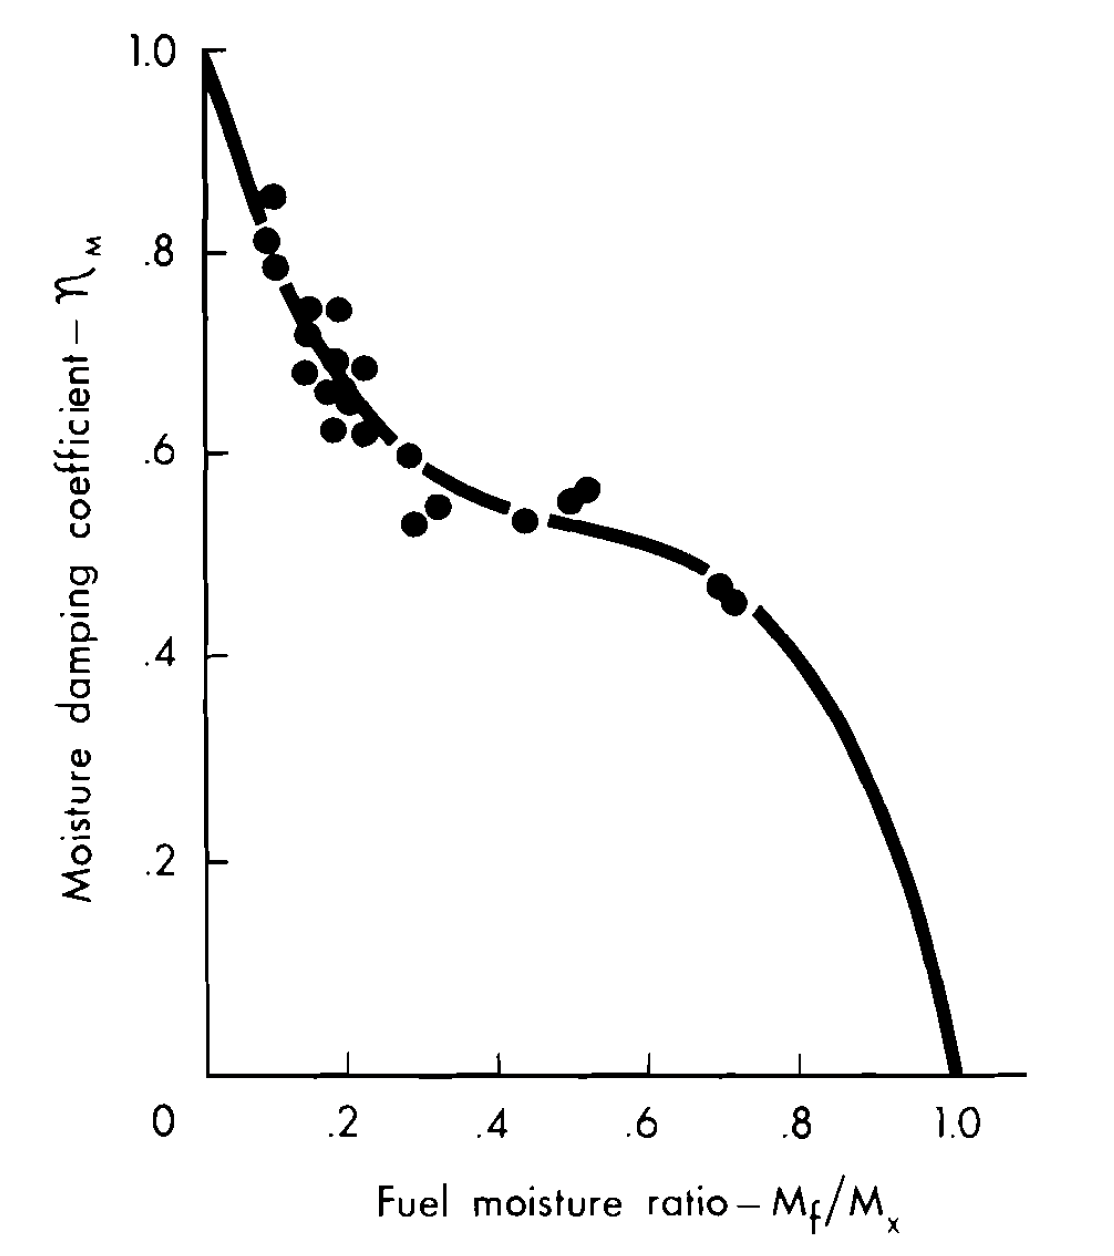
\includegraphics[scale = 0.40]{/Users/jeremybenik/Research_Files/164/Assignments/draft/Images/Rothermel/moisture_damping.png}
  \caption{Determining the moisture damping coefficient}
  \label{rothermel_moisture_damping}
\end{figure}

 \indent To find the mineral damping coefficient, the authors assumed the ratio of the "normalized decomposition rate would be the same as the normalized reaction intensity" (Rothermel, 1972). They then used the maximum decomposition rate and found the mineral content was at 0.0001 which was the lowest fractional mineral content for natural fuels. By then looking into silica-free ash, the authors were able to create another plot as seen in \ref{rothermel_mineral_damping}. They then found the equation fitting the curve and set that as the mineral damping coefficient. To find the damping coefficient, all the user needs to input is the effective mineral content (silica free). \\
 \begin{figure}
  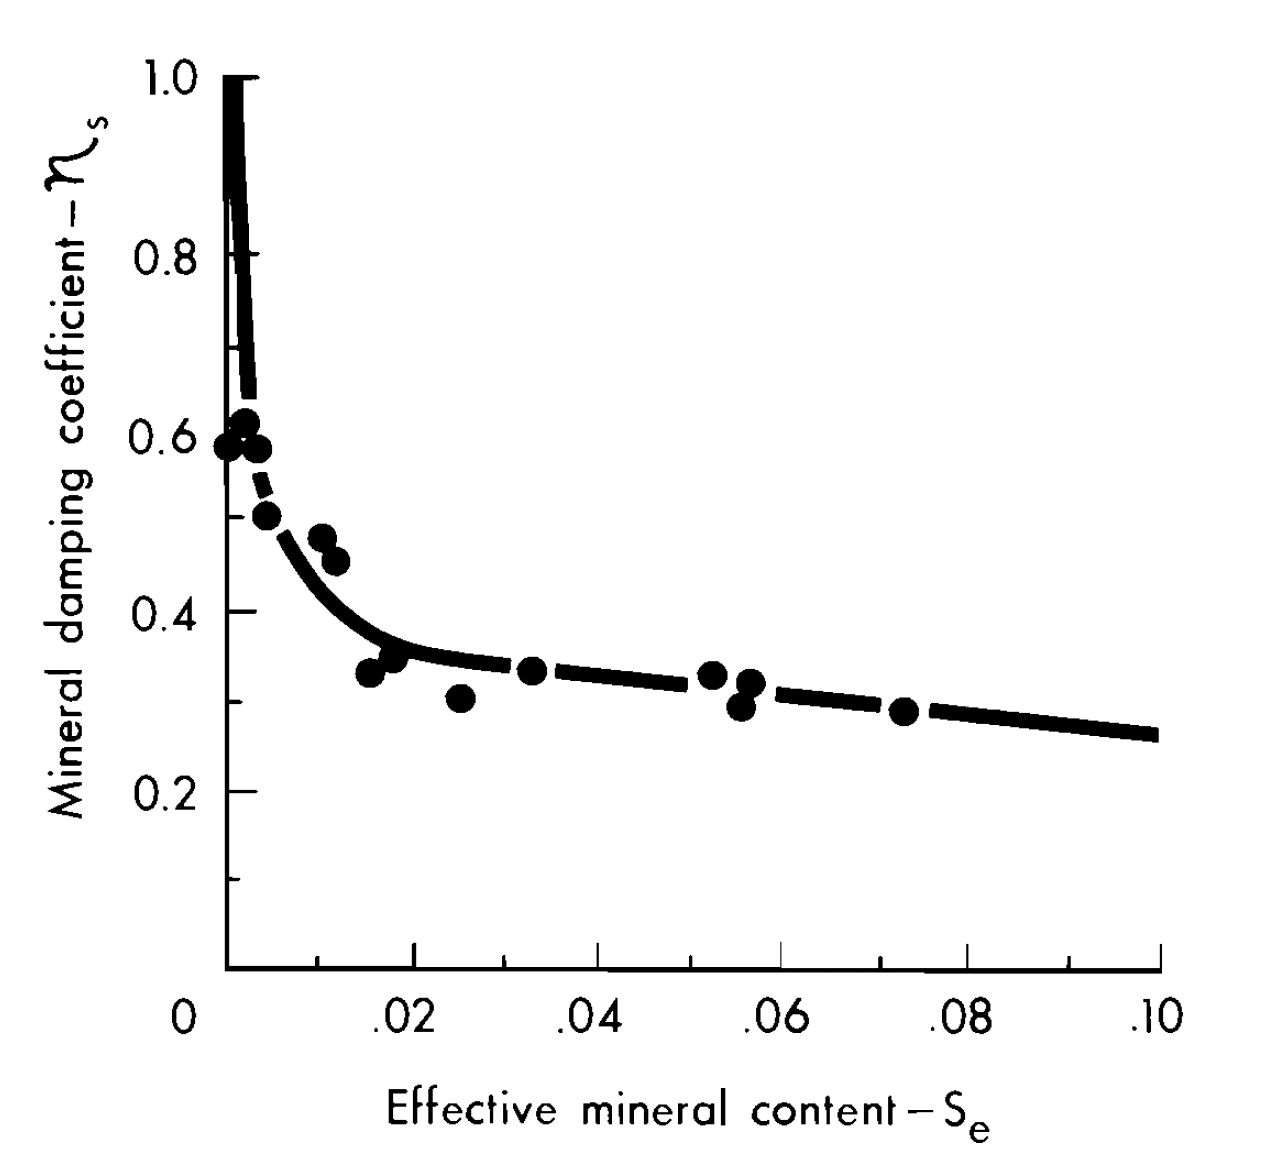
\includegraphics[scale = 0.40]{/Users/jeremybenik/Research_Files/164/Assignments/draft/Images/Rothermel/mineral_content.png}
  \caption{Determining the mineral damping coefficient }
  \label{rothermel_mineral_damping}
\end{figure}
 \subsubsection{Fuel Packing Ratio and Surface Area to Volume Ratio}
 \indent The last parameters are the fuel packing ratio and the surface area to volume ratio. Both of these are fuel properties and need to be specified within the fuels parameter in the inputs to work. These parameters are necessary as they determine how intense a fire may spread. With a high packing ratio, there will be a low air-to-fuel ratio and this will make it difficult for the flame to penetrate to the top of the fuel. However a more sparse fuel bed will result in a low intensity fire as there will be significant heat losses between the fuel and flame. Finding the optimal packing ratio to achieve the maximum fire intensity is a challenging task as it is likely different for each fuel. the packing ratio can be defined by \ref{Equation 8}
 \begin{equation}
 	\beta = \frac {\rho _ b } {\rho _ p} 
 \end{equation}
Where: \\
$\beta$ = packing ratio, dimensionless. \\
$\rho _ b$ = fuel array bulk density, lb./ft$^3$ \\
$\rho _ p$ = fuel particle density, lb./ft$^3$ \\

\indent The surface area to volume ratio (SAVR) for fuels is used to quantify the fuel particle size can be represented by \ref{Equation 9}
\begin{equation}
	\label{Equation 9}
	\sigma = \frac {4} {d} 
\end{equation}
 Where d = the diameter of the circular particles or edge length of square particles, ft. \\
 \subsubsection{Fitting Missing/Unknown Parameters Through Experimentation}
 \indent With the whole model setup, the authors next task was to find the parameters that could only be found through experimentation. This includes the parameters in the reaction velocity, and the slope and wind coefficients. To find the reaction velocity parameters, the authors setup multiple fuel beds on weighing platforms so the weight of the fuel could be constantly measured. This allowed them to determine how fast the fuel was burning since they had multiple weight sensors at each part of the fuel. With this knowledge, they found that the mass loss rate related to the net initial fuel loading, reside loading, and the width of the weighing platform. Combining this with equation \ref{Equation 6} yields \ref{Equation 10}
 \begin{equation}
 	\label{Equation 10}
 	\Gamma = \frac {\dot m } {w_n RW \tau _ R} 
 \end{equation}
 Where: \\
 $\dot m$ = mass loss rate obtained from the weight loss data. \\
 \indent With this final equation, it can then be combined with \ref{Equation 7} to get the potential reaction velocity and have it now correlated with the physical features of fuel. 
 \begin{equation}
 	\label{Equation 11}
 	\Gamma ^ {'} = \frac {\Gamma} {\eta _ M \eta _ S}
 \end{equation}
 
\indent With all the equations finally formulated, experiments were then performed using this model and comparing it to the observed rate of spread. The first parameter tested within the model to observations is the reaction velocity. In particular, they wanted to find the optimum packing ratio and the optimum reaction velocity. After numerous experiments, they found there is an optimum fuel load for each fuel size. To incorporate this into the model, they combined the maximum reaction velocity with the regular reaction velocity equation and an arbitrary variable A was inserted to better fit the observation. The final equation for the reaction velocity then became: 
\begin{equation}
	\label{Final Reaction Velocity}
	\Gamma ^ {'} = \Gamma ^ {'}_{max} (\frac {\beta} {\beta _ {op}}) ^ {A} exp[A(1 - \frac {\beta} {\beta _ {op}})]
\end{equation}
Where: \\
A = $\frac {1} {(4.77 \sigma ^ {.1} - 7.27)}$\\
\indent These equations were designed to fit not only the dependent variables but also the data obtained in their experimentation. These equations are specifically made for reasonable output values even when the input values may be extreme so the model should never go to negative infinity or go negative. \\
\indent Next is the propagating flux. To first evaluate the equations, the authors assumed no wind and no slope to make formulating these equations much more simple. The initial equation for the propagating flux can be seen in equation \ref{Propagating flux with i0}.
\begin{equation}
	\label{Propagating flux with i0}
	(I_P)_o = R_0 \rho _ b \epsilon Q_{ig}
\end{equation}
Where $\epsilon$ is a ratio between the propagating flux and reaction intensity. To get the value for $\epsilon$, the authors used the fuel packing ratio from 3 fuel sizes and fit the data to the curve in Figure \ref{rothermel_eta}
\begin{figure}
  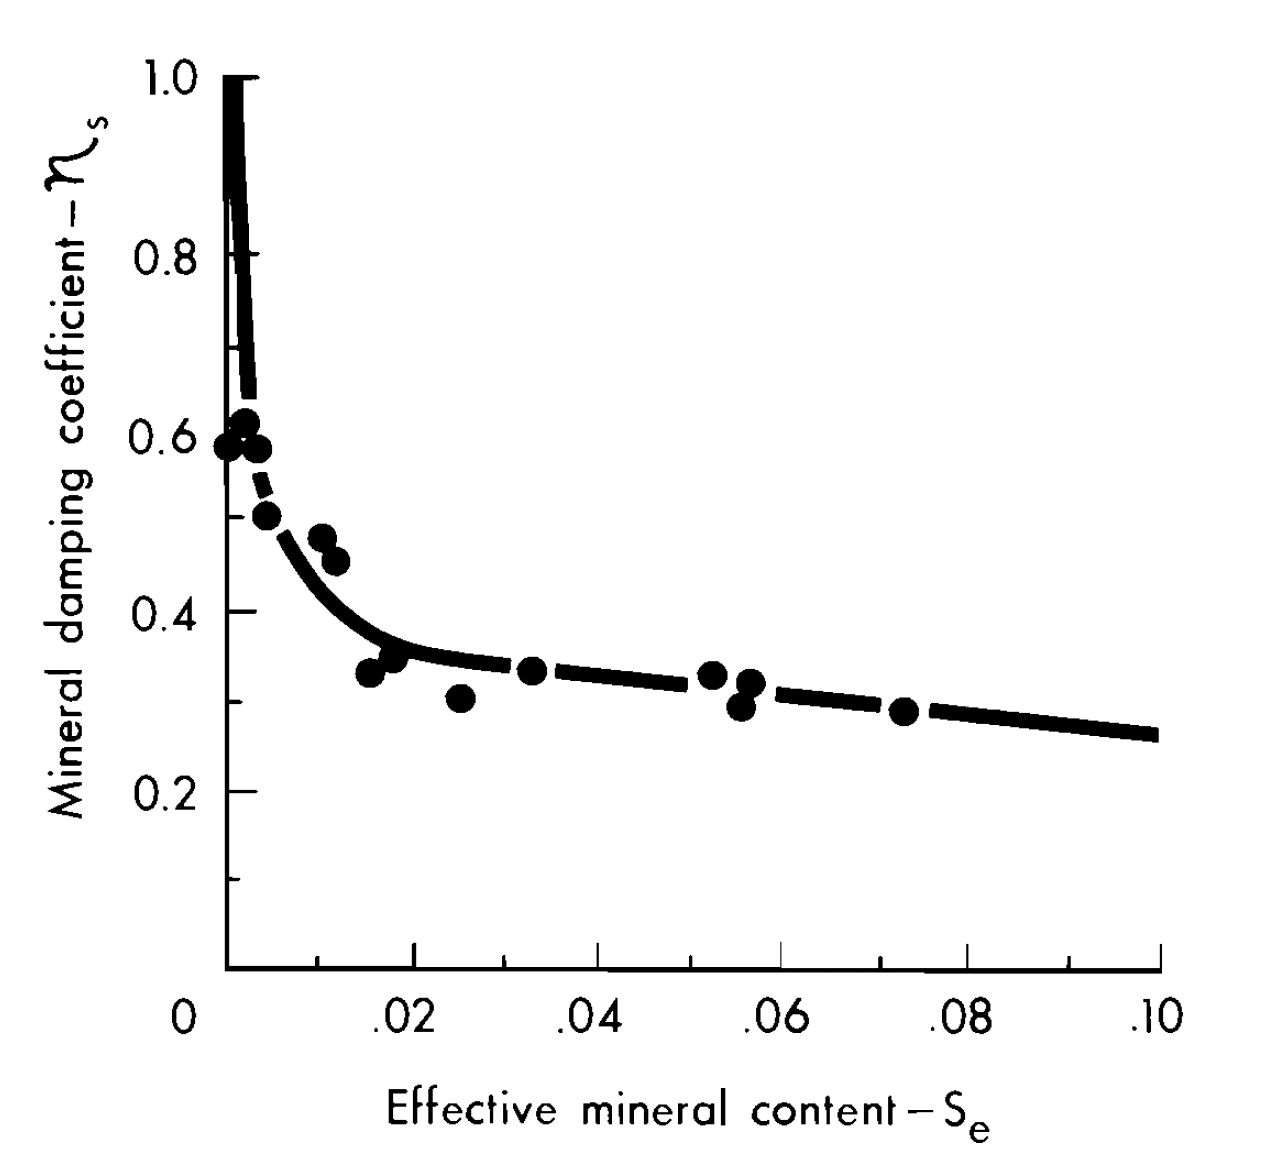
\includegraphics[scale = 0.40]{/Users/jeremybenik/Research_Files/164/Assignments/draft/Images/Rothermel/mineral_content.png}
  \caption{Determining the mineral damping coefficient }
  \label{rothermel_mineral_damping}
\end{figure}
\subsubsection{Wind and Slope Coefficients}
\indent To evaluate the wind and slope coefficients, the authors assume that the fuel would remain constant. After performing multiple experiments with varying fuel beds at different wind speeds and using field data, they got the wind coefficient to be a function of SAVR along with many other constants to match observed data. The wind coefficient can be seen in \ref{wind coefficient}. The slope coefficient was calculated by performing experiments on fuel beds at different slopes. They then found a correlation of the data collected from the experiments and used that as the slope factor and this can be seen in \ref{Slope coefficient}
\begin{equation}
	\label{wind coefficient}
	\phi _ W = C U^{B} (\frac {\beta} {\beta_{op}}) ^ {-E}
\end{equation}
\begin{equation}
	\label{Slope coefficient}
	\phi _ S = 5.275 \beta ^ {-.3} (tan \phi)^{2}
\end{equation}
Where: \\
C = $7.47 \exp(-0.133 \sigma^{0.55})$ \\
B = $0.02526 \sigma^{0.54}$\\
E = $0.715 \exp(-3.59 * 10^{-4} \sigma)$\\
\subsubsection{Final Rate of Spread Equation}
\indent The final ROS equation was finally done and it now incorporates both slope and wind components and is able to be used operationally. There is no longer any calculus needed or any complex calculations. The final equation can be seen in \ref{rothermel final ROS}. 
\begin{equation}
	\label{rothermel final ROS}
	R = \frac {I_R \zeta (1 + \phi _ W + \phi _ S )} {\rho _ b \epsilon Q_{ig}}
\end{equation}
\subsection{Balbi Model}
\subsubsection*{2007 Balbi Model}
\indent With multiple versions of the Balbi model, the first model will be discussed followed by the newest version to see how much the model has changed since the original model. the Balbi model is a fully physical model so there will be no observations used in this paper, only physical properties of fires.
\subsubsection{Simplified Flow and Flame Tilt Angle}
\indent The first parameter in the Balbi model is the simplified flow and the flame tilt angle. These parameters are first calculated assuming no slope and no wind conditions (like with Rothermel initially). They assume the main effect of the flow that must be accounted for is the tilting of the flames under wind and/or slope conditions (Balbi, 2007). However for the initial study, they will assume that under no wind and no slope conditions the flame tilt angle $\gamma$ equals $\beta _ w$ which results from the buoyancy and the wind. $\beta _w$ is given by:
\begin{equation}
	\label{beta_w}
	\tan \beta _ w = \frac {\nu _ w} {u_{fl}}
\end{equation}
Where:\\
 $\nu _ w$ and $u_{fl}$ represent the free stream wind speed and the upward gas flow velocity in still air at mid flame height. \\
\indent However with a slope, $\gamma$ changes as the gas velocity changes due to indrafts ($\nu _ s$) and the slope angle ($\alpha _0$). Their relationship can be seen in \ref{gamma} and \ref{tan_beta}
\begin{equation}
	\label{gamma}
	\gamma = \alpha + \beta _ s
\end{equation}
\begin{equation}
	\label{tan_beta}
	\tan \beta _ s = \frac {\nu _ s} {u_{fl}}
\end{equation}
\indent For circumstances where there are both wind and slope conditions, they assume the gas velocity induced from the slope factor is negligible in regards to the wind speed.
\subsubsection{Simplified Flame Sub-Model}
\indent To be able to calculate $\nu _ w$ and $u_{fl}$ and keep the model "faster than real time" (Balbi, 2007), many simplifying assumptions are made to generate a simple model. To do this, the authors split the flame into two different categories, the flame base and the flame body. They split the calculation up into 6 sections: Flame height, State Equation, Vertical Momentum Equation, Mass Balance, Stoichiometric Ratio, and Thermal Balance. l is the depth and H is its height. The authors used a previous relationship by Sun et al. (2003):
\begin{equation}
	\label{Flame height}
	H = H^{*} Q^{\frac {2}{5}} = H^{*}(\Delta h_{fu} \sigma _{fu} c) ^{\frac {2}{5}}
\end{equation}
Where:\\
H is the flame height.\\
Q is the rate of heat release per unit length of fire front. \\
$H^{*}$ is a parameter to fit. \\
$\Delta h_{fu}$ is the heat of combustion of the vegetative fuel. 
$\sigma _{fu}$ is the surface mass. \\
c is the rate of fire spread.  \\ 
To better visualize this, refer to Figure \ref{Balbi_flae_height_diagram}.
\begin{figure}
  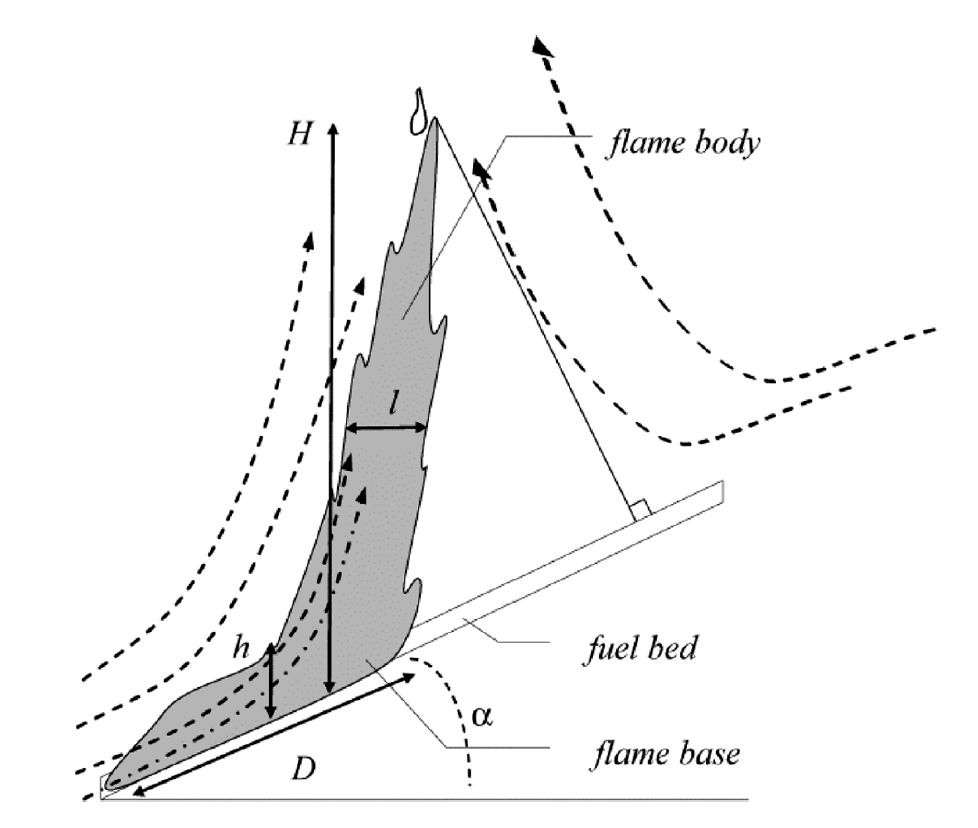
\includegraphics[scale = 0.40]{/Users/jeremybenik/Research_Files/164/Assignments/draft/Images/Balbi/balbi_flame_height.png}
  \caption{Diagram of the different characteristics of the flame in the 2007 Balbi Paper}
  \label{Balbi_flae_height_diagram}
\end{figure}

\indent As seen in Figure \ref{Balbi_flae_height_diagram}, there is a vertical component to the flame. To calculate this component, they first neglect the shear stresses in the gas and instead use buoyancy as the main mechanism involved in the vertical momentum. this is given by: 
\begin{equation}
	\label{Vertical momentum Balbi}
	\rho _ g \frac {\partial u} {\partial t} = (\rho _a - \rho _g) g
\end{equation}
\indent To solve for this equation, simple integration along the flame length results in the gas velocity at mid flame, $u_{fl}$
\begin{equation}
	\label{gas velocity}
	u_{fl} = Q ^ {\frac {1}{5}} \sqrt{(\frac {T_{fl}} {T_a} - 1) g H^{*}}
\end{equation}

\indent Mass balance is kept simple for the whole flame structure based on the geometry of the flame. In slope and wind conditions, the rate of air entrainment is considered negligible in ass balance. With this assumption, the continuity equation per unit length of the fire can be used and is given by:
\begin{equation}
	\label{mass balance balbi}
	\rho_g u_{fl}l = \rho_{ga} h \nu _u + D \dot{\sigma} _ {fu}
\end{equation}
Where the left hand side of the equation is the rate of mass loss from the flame body, $ + D \dot{\sigma} _ {fu}$ is the rate of air entrainment upward in the flame, and $D \dot{\sigma} _ {fu}$ is the rate of mass increase due to the thermal degradation of the vegetation. \\
\indent The stoichiometric ratio involves the rate of air entrainment upward in the flame and how that is proportional to the rate of mass incoming from thermal degradation, $\upsilon$ being the stoichiometric ratio (Balbi, 2007). 
\begin{equation}
	\label{stoich ratio}
	\rho _ a h \nu _ u = \upsilon D \dot{\sigma} _ {fu}
\end{equation}
\indent The last parameter in the flame sub model is the thermal balance. The thermal balance calculates the temperature of the flame and has the same assumptions as the continuity equations. After simplifications and rearranging the initial equation, as well as assuming the specific heat is held constant in the flame, fuel gases, and that the fuel gases are emitted near the ambient temperature, the equation for the flame temperature becomes:
\begin{equation}
	\label{flame temp balbi 2007}
	T_{fl} = T_a + \frac {(1 - \chi) Q}{(\upsilon + 1) D \dot{\sigma} _ {fu} c_{pg}} = T_a + \frac {1 - \chi) \Delta h _ {fu} }{(\upsilon + 1) c_{pg}}
\end{equation}
\subsubsection{Simplified radiation Sub-Model}
\indent When a fire front spreads, there is a radiant heat flux impinging on the unburnt fuels ahead of the flame front (Balbi, 2007). This component is split up into two different components. The radiative component from the flame base, and the flame body radiation. For the flame base radiation, they assume the emissivitiy of the flame base is equal to unity (Balbi, 2007), which results in:
\begin{equation}
	\label{R_b 2007}
	R_b = \sigma T^{4}_{fl} \mathrm{d}(\delta - x)
\end{equation}
Where "$T_{fl}$ is the flame temperature (calculated in equation \ref{flame temp balbi 2007}), $\delta$ = $4/ \alpha _{fu} \zeta _ {fu}$ is the mean penetration distance of radiation within the fuel bed. x is the coordinate in space normal to the fire front and d represents the fuel depth" (Balbi, 2007). \\
\indent When flames are on a slope or under windy conditions, the flame is brought closer to the unburnt fuel, which preheats the fuels more than if the flame were vertical. The base radiation would stay the same under any conditions however. The amount of radiation is a complex calculation however since the amount of radiation reaching the unburnt fuel from the flame body must be integrated the length of the flame as well as using an inverse square law to find the distance r between the two areas. To reduce this equation to be used in a simplified model that is "faster than real time" (Balbi, 2007), an assumption that the fire front is a flame panel with height H and infinite width from a surface fuel element (Balbi, 2007). The equation then becomes:
\begin{equation}
	\label{flame_base_2007}
	R_{fl} = \epsilon_{fl} \sigma \frac {T^{4}_{fl}} {2} (1 - \cos \theta)
\end{equation}
Where $\theta $ is the angle between the base of the flame panel and the element of surface fuel. 
\subsubsection{Preheating Sub-Model}
\indent This is the last submodel in the 2007 Balbi model. In this submodel, the authors introduce the Relationship for the Rate of Spread under Low Speed Regimes, Relationship for the ROS under High Speed Regimes, and a simplified model of fire spread under high speed regimes. The major assumption made here is the radiation is denoted as the prevailing form of heat transfer in fire spread. Like with the Rothermel model, calculations are first made with no wind no slope conditions to simplify calculations and those parameters are added in later. With no wind no slope conditions, the fire propagation will remain relatively constant  for a given fuel. Whereas with wind or a slope, that will introduce a flame tilt and thus preheat the fuels ahead of the fire much more effectively. The base equation for the preheating sub model is as follows:
\begin{equation}
	\label{preheating sub mode 2007}
	\sigma _ {fu} c _{pfu} \frac {\mathrm{d} T_{fu}} {\mathrm{d} t} = R_b + R_{fl} - \Delta h_w \frac {\mathrm{d} \sigma _ w } {\mathrm {d} t}
\end{equation}
Equation \ref{preheating sub mode 2007} represents the thermal balance for the unburned fuel ahead of the fire front. \\
\indent Under a low speed regime, $\gamma$ will likely remain close to 90$^{\circ}$ as there is no slope or little to no wind pushing the flame closer to the unburnt fuel. As a result, $R_{fl}$ can be neglected in this case and equation \ref{preheating sub mode 2007} can be solved with neglecting the flame body radiation. After substitutions and some manipulation of the equation above, the resulting equation is:
\begin{equation}
	\label{low regime ros}
	c_1 = \frac {\sigma T^{4}_{fl} \mathrm {d} \delta ^ 2} {2 \sigma _ {fu} (c_{pfu}(T_{ig} - T_a) + \Delta h _ w \eta)}
\end{equation}
Where:\\
$c_1$ = constant ROS. 
dx = $c_1 \mathrm{d}t$
$\eta$ = moisture content defined by $\eta = \sigma _ w / \sigma _ {fu}$ \\
\indent On the other hand, with a high speed regime, the flame body radiation is assumed to be the main form of heat transfer to the unburned fuels. As a result, $R_b$ is negligible and can be omitted in these calculations. By assuming that the ROS is constant over the space interval from 0 to $H \sin \gamma$, equation \ref{preheating sub mode 2007} can be integrated and solved as:
\begin{equation}
	\label{high speed regimes}
	c_h = c_l  + \frac {\epsilon _{fl} \sigma T^{4}_{fl} H} {2 \sigma _ {fu} (c_{pfu}(T_{ig} - T_a) + \Delta h _ w \eta)} (1 + \sin \gamma - \cos \gamma)
\end{equation}
\indent Sine $c_l$ is negligible as the flame body is the main contributor to the rate of spread, it can be removed from equation \ref{high speed regimes}\\
\indent The final parameter is the simplified model of fire spread under high-speed regimes. To calculate this, first the authors define how much heat is actually transferred from the flame to the unburnt fuel. This is given by:
\begin{equation}
	\label{high speed regimes 2007}
	\epsilon_{fl} \sigma T^{4}_{fl} = \chi Q / H
\end{equation} 
To further reduce this model to reach the final form, the fraction of radiation $\chi$ decreases with flame width according to a parameter q that must be fitted in experimentation later on. \\
\indent By combining all the above equations together, both no slope no wind and conditions with slope and wind, it results in a large series of nonlinear equations. Solving these is not an issue however as the equations have been simplified down and can be solved "faster than real time" (Balbi, 2007). By simulating the fire front shape, the authors found that to find the rate of spread at a specific point, the model needs to be run at every location on the fire front. Usually, a grid would be constructed to help in solving this, but the authors utilized Mathematica and used that to represent the fire front shape on a three dimensional domain. By using this technique, the computational time is lower than real time (Balbi, 2007). Now all that is left for the model is validating it using lab and experimental burns and fitting parameters. Some of the parameters they found remained relatively constant throughout the different burns (q = 3), but the other parameters varied with different fuels characteristics. Such as A depends mainly on the fuel moisture,$b_s$ and $b_w$ depend on the fuel surface mass. $c_l$ (low rate of spread) depends on the optical depth, moisture content and the volume mass. \\
\subsubsection*{2022 Balbi Model}
\indent With many other revisions to this model (such as the 2009 paper, 2020 paper), this model has undergone a lot of change and this will be evident by the amount of change in the 2022 Balbi paper. The most notable difference is a convective component was added to the model. Before, the model only considered the flame base radiation and the flame body radiation, but now there is a convective component that helps spread the fire in a similar location as the base radiation according to Figure \ref{Balbi_flame_diagram}. This component is based on the inflow of hot gases from the lower part of the flame base. \\
\begin{figure}
  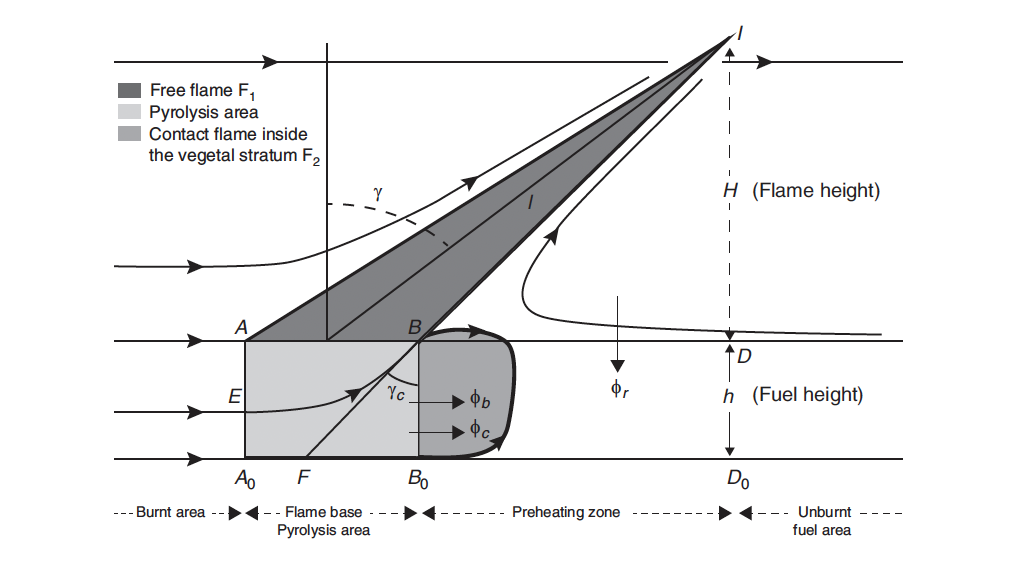
\includegraphics[scale = 0.60]{/Users/jeremybenik/Research_Files/164/Assignments/draft/Images/Balbi/balbi_diagram.png}
  \caption{Diagram showing the idealized scenario of the flaming zone}
  \label{Balbi_flame_diagram}
\end{figure}
\indent Figure \ref{Balbi_flame_diagram} is essentially what the whole model follows. There is the flame body radiation, flame base radiation, and the convective radiation. The convective component was originally introduced in the 2020 Balbi paper. That paper was created in a laboratory setting and was advertised as able to be used in a field setting. After extensive testing, the developers created another model (the 2022 model) and changed some parameters (as well as introduced more). \\
\indent Since the other two parameters have been discussed, those will not be covered in this section. Instead, the main focus will be on the convective component as that has proven to be one of the most sensitive parameters within the model. The convective component is initially modeled as:
\begin{equation}
	\label{convection intro}
	\phi _ c = \frac {\Delta H} {2 \tau _ 0} \sigma s min(h, \delta) \tan \gamma _ c
\end{equation}
Where: \\
$\Delta H$ and $\tau _ 0$ are the heat of combustion of pyrolysis gases and the flame residence time parameter (Balbi, 2022).\\
\indent The angle $\gamma _ {c}$ is defined as :
\begin{equation}
	\tan \gamma _ {c} = \tan \alpha + \frac {U(L)} {u_{c}}
\end{equation}. 
Where U(L), $u_c$, and $\alpha$ are horizontal wind speeds at point B (Balbi, 2022). U(L) is further expressed as a function of the wind velocity at mid flame and accounts for drag forces. After some simplifications and substitutions, the authors found the final equation for the convective component $R_c$: \\
\begin{equation}
	\label{convective component}
	R_c = a_M min(\frac {W_0}{50}, 1) \frac {\Delta H \rho _ a T_a s \sqrt{h}}{2q(s_t + 1) \rho _ v T} (\frac {(s_t + 1) \rho _ v T}{\tau _ 0 \rho _ a T_a} min(S, \frac {2 \pi S}{S_t} \tan \alpha + U \exp (- \frac {\beta _ t}{min(\frac{W_0}{50}, 1)} R))
\end{equation}
Where: \\
$R_c$ = Contribution of convection to the ROS ($m/s$).\\
$a_M$ = fitted model parameter. \\
$W_0$ = Ignition line width (m). \\
$\Delta H$ = Heat of combustion of the pyrolysis gases ($J / kg$). \\
$\rho _ a$ = Air Density ($kg/m^3$) \\
$T_a$ = Air Temperature (K) \\
h = fuel bed depth (m) \\
q = Ignition Energy ($J / kg$) \\
$s_t$ = air Pyrolysis gases mass ratio in the flame body. \\
$\rho _ v$ = Fuel Density ($kg/m^3$) \\
T = Mean flame temperature (K)\\
$\tau _ 0$ = Flame residence time parameter ($s / m$) \\
S = Leaf area by square meter ($m^ 2 / m^2$) \\
$\alpha$ = Terrain slope angle (degrees)\\
U = Sum of normal component (to the fire front) of the natural wind velocity and fire generated inflow coming from the burnt area ($m / s$). \\
$\beta _ t$ = Total packing ratio. \\
R = Rate of Spread ($m / s$). \\
\subsection{Comparison of the Two Models}
\indent To test these two models, the two models were places under the same fuel categories and the same environmental conditions. Using the Kolgerberg dataset from the Van Wilgen experiment, a separate fuels category was created for the fuels used in this field study. The fuel in their study was the South African Fynbos fuels. In their experiment (for the first experiment which is the one that will be extensively tested), there was a small wind of 1.5m/s and a slope of 3 degrees. The fuel moisture was at 3 percent and the air temperature was 297.4 K. The observed rate of spread in this experiment was 0.36 m/s. The Balbi code was originally using the 2018 paper, but has since been updated to the 2020 paper with the help of Adam Kochanski and John Stuart. This code was made to fit the same values as the developers of the Balbi model using the Kolgerberg experimental dataset, whereas there was one modification to the Rothermel model. In the Rothermel model there is a parameter that takes the maximum of the ROS up until 6 m/s. To better understand what the model does in extreme conditions this was left out so there is no cap at 6m/s. Some assumptions in these experiments are the air temperature will remain constant, the ignition line width will remain constant at 50m (this was later removed in the 2022 paper). With these conditions, the models can be properly tested. All plots will plot the same variables despite changes or not in them. The reason for this is so any change in the rate of spread can be easily identified (such as if the base radiation is the main contributor to the ROS or the wind coefficient). 
\subsubsection{Wind Speed}
% Wind Speed
\begin{figure}
\centering
  \includegraphics[scale = 0.13]{/Users/jeremybenik/Research_Files/164/Assignments/draft/Images/Rothermel/Wind_Speed.png}
  \includegraphics[scale = 0.20]{/Users/jeremybenik/Research_Files/164/Assignments/draft/Images/Balbi/Wind_Speed.png}
  \caption{Comparison of the Balbi model and Rothermel model under wind speeds from 0-20m/s}
  \label{Wind Speed}
\end{figure}
\indent In Figure \ref{Wind Speed}, the ROS in the Rothermel model reaches close to 20m/s which is not a valid ROS value. In the code there is a point where it caps out at 6m/s, but this was removed for testing purposes to determine how much the ROS would increase without a cap on it. The main contributor to the ROS is the wind coefficient which follows the trend of the ROS almost exactly. The other parameters used to calculate the ROS do now change as those plots are blank. The Balbi model on the other hand follows a similar story to the Rothermel model, however the ROS value is more reasonable as it reaches a little over 2.5 m/s, indicating this model is much more reasonable in extreme situations. The main component driving the rate of spread in this model is the convective component which is only about 0.5 m/s lower than the overall ROS. The flame body radiation component also begins to contribute more with a greater wind speed. This is likely due to with a greater wind speed, that is pushing the flame closer to the unburnt fuel, lowering $/gamma$ and more effectively preheating the fuel. 
% Slope
\subsubsection{Slope}
\begin{figure}
\centering
  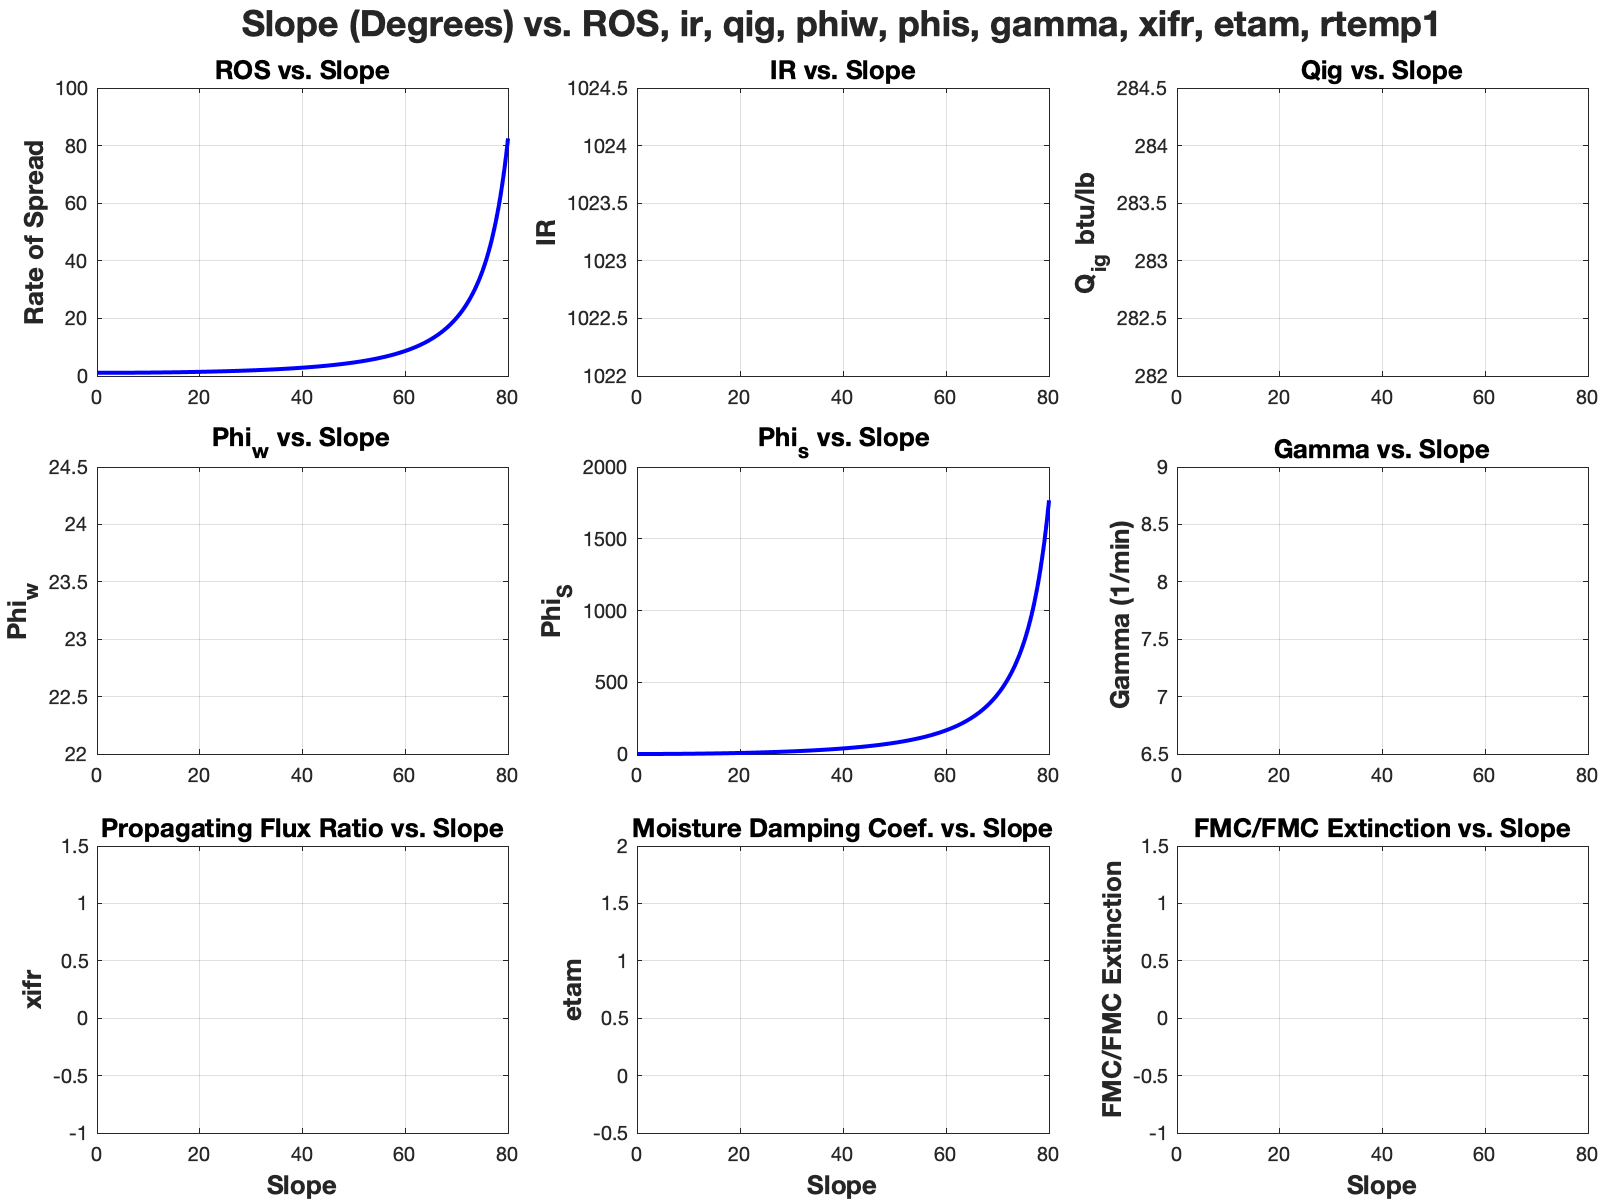
\includegraphics[scale = 0.13]{/Users/jeremybenik/Research_Files/164/Assignments/draft/Images/Rothermel/slope_rothermel.png}
  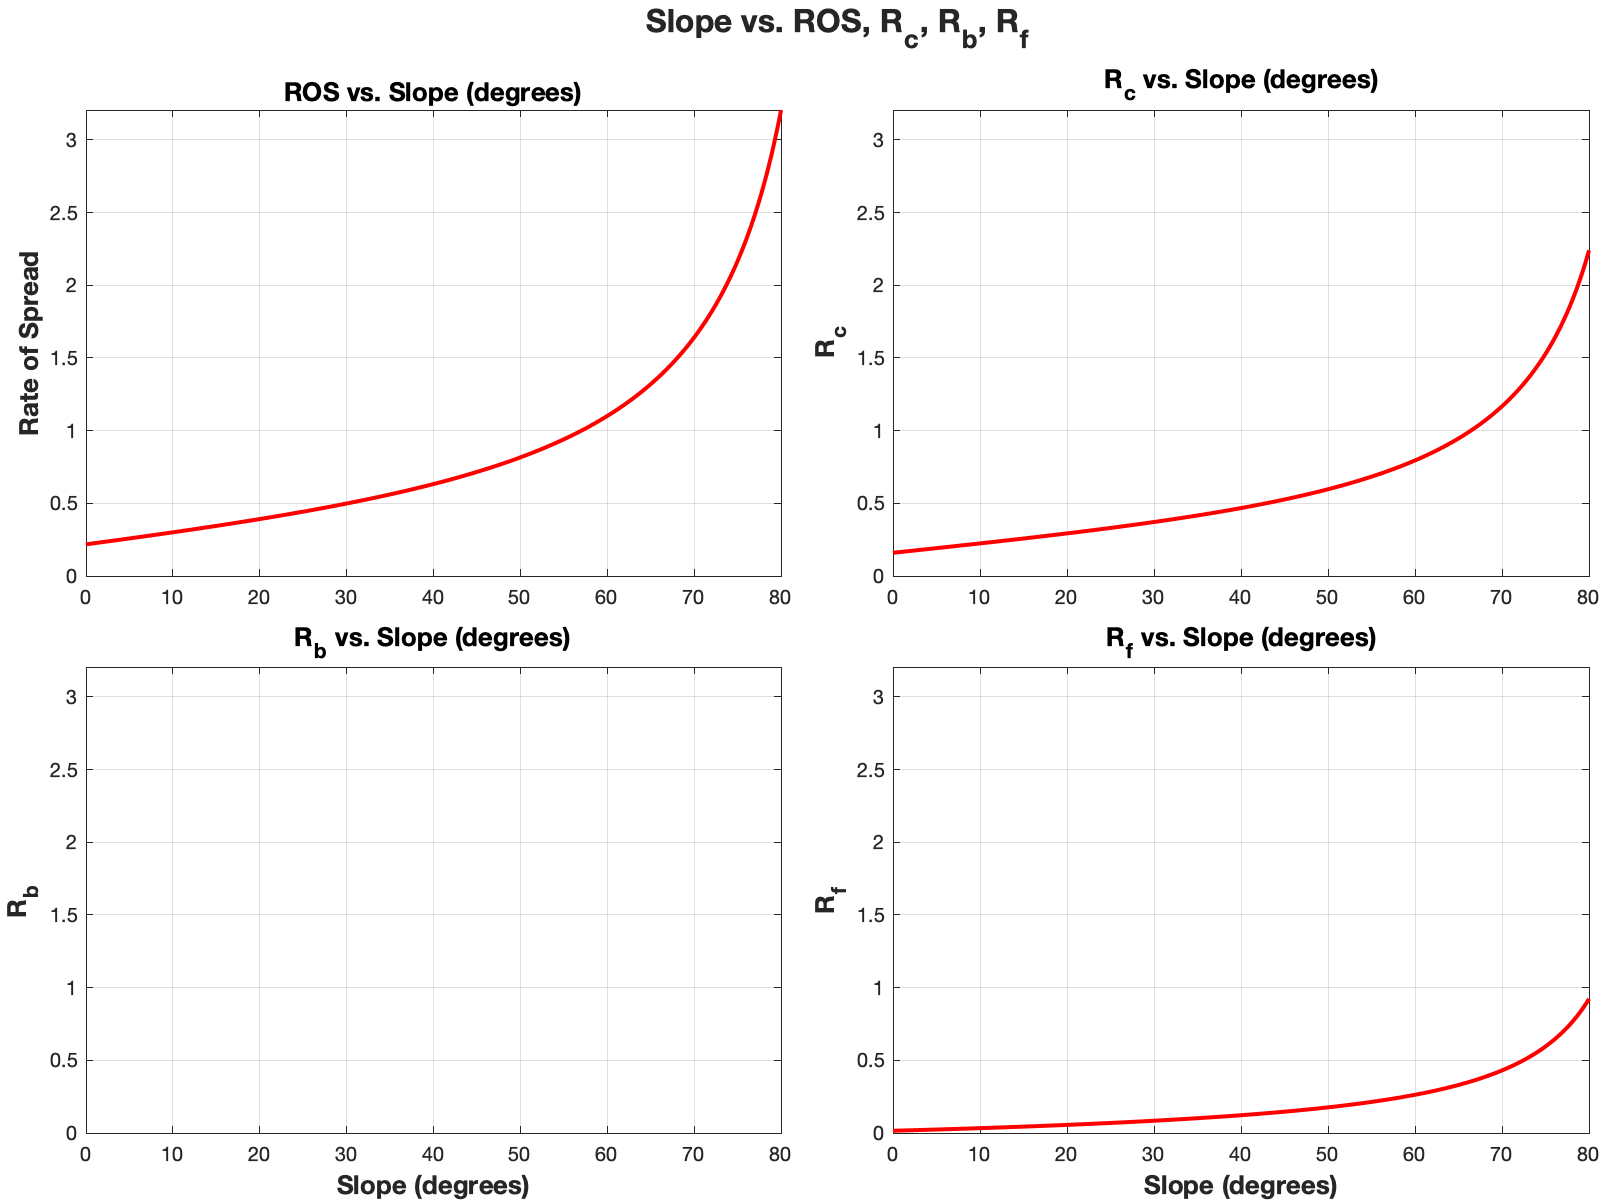
\includegraphics[scale = 0.20]{/Users/jeremybenik/Research_Files/164/Assignments/draft/Images/Balbi/Slope.png}
  \caption{Comparison of the Balbi model and Rothermel model under varying slopes from 0-80 degrees}
  \label{Slope}
\end{figure}
\indent The next component tested is the slope. In Figure \ref{Slope} the two ROS models follow the same exponential pattern, but like in Figure \ref{Wind Speed} the Rothermel model produces unreasonable results as the slope approaches 80 degrees. The slope coefficient is the main contributor for the ROS as the curves are identical. On the other hand the Balbi model remains at reasonable values with the ROS around 3m/s with the convective coefficient being the main driver for the ROS. With a greater slope, the flame body radiation also increases like with \ref{Wind Speed}

% Fuel Moisture With Slope
\subsubsection{Fuel Moisture}
\begin{figure}
\centering
  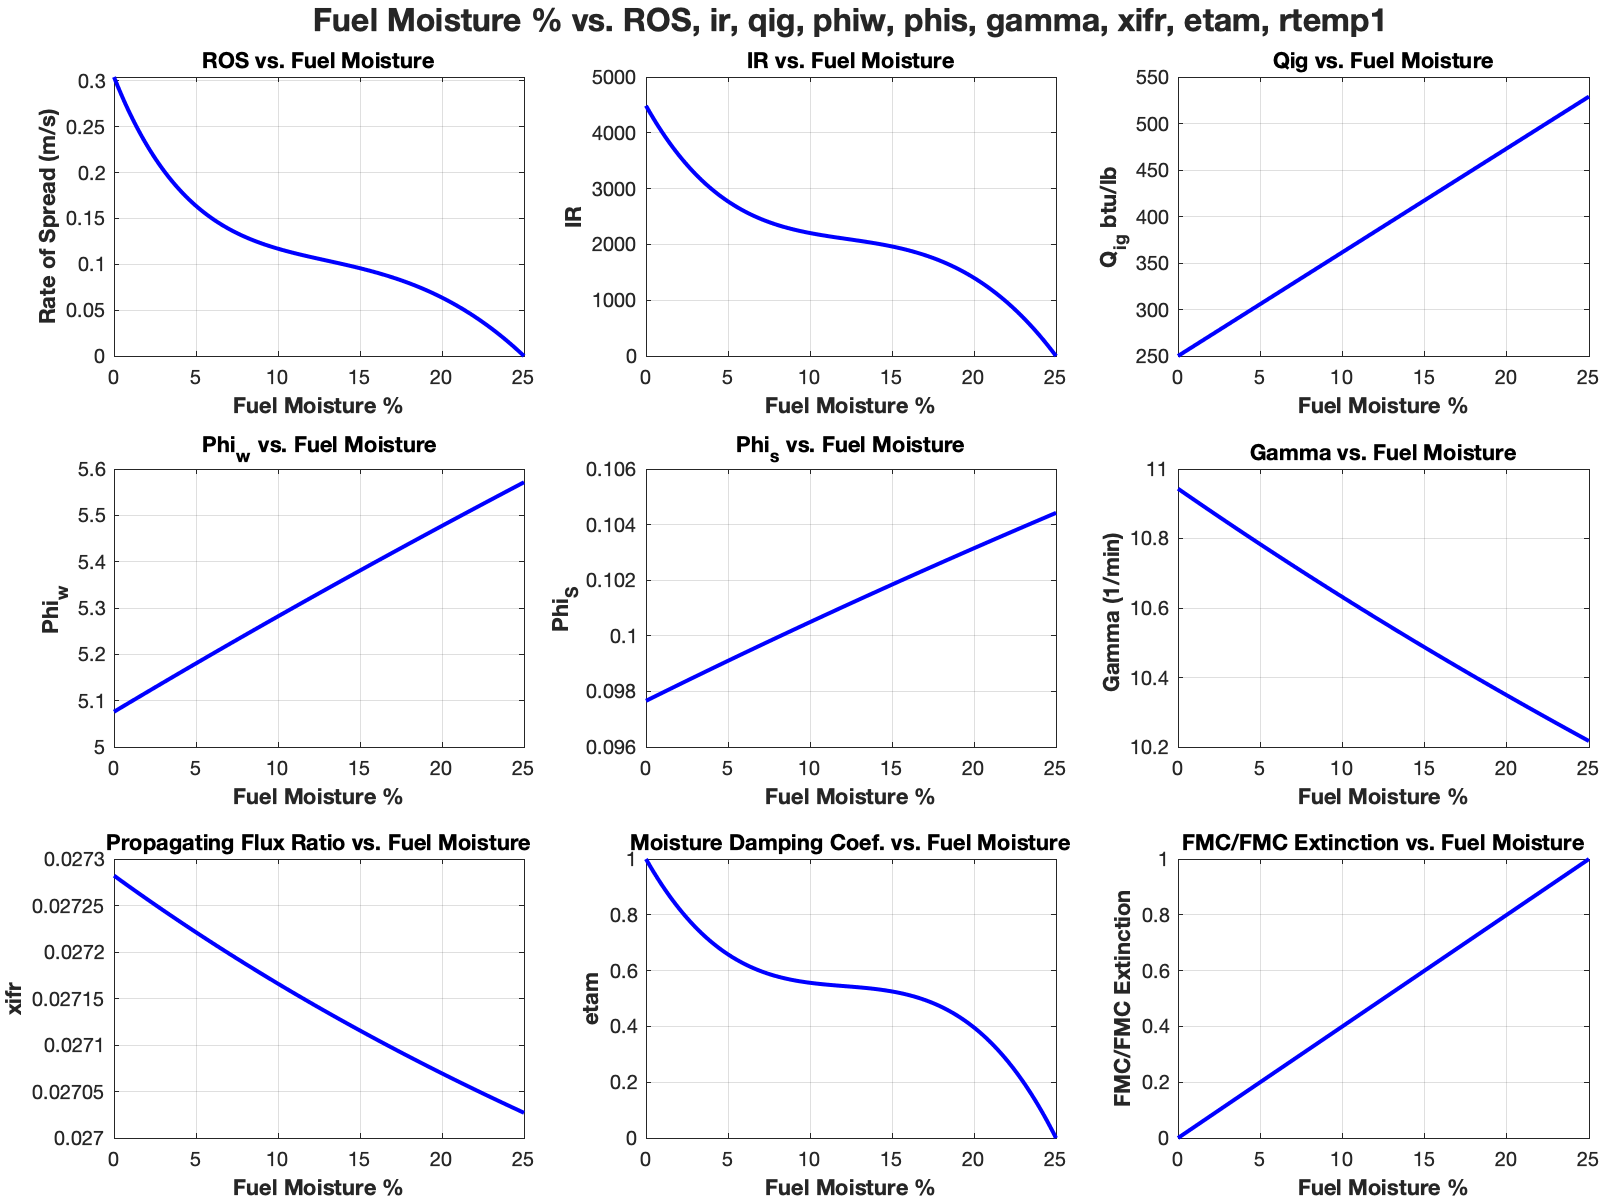
\includegraphics[scale = 0.13]{/Users/jeremybenik/Research_Files/164/Assignments/draft/Images/Rothermel/FMC_rothermel.png}
  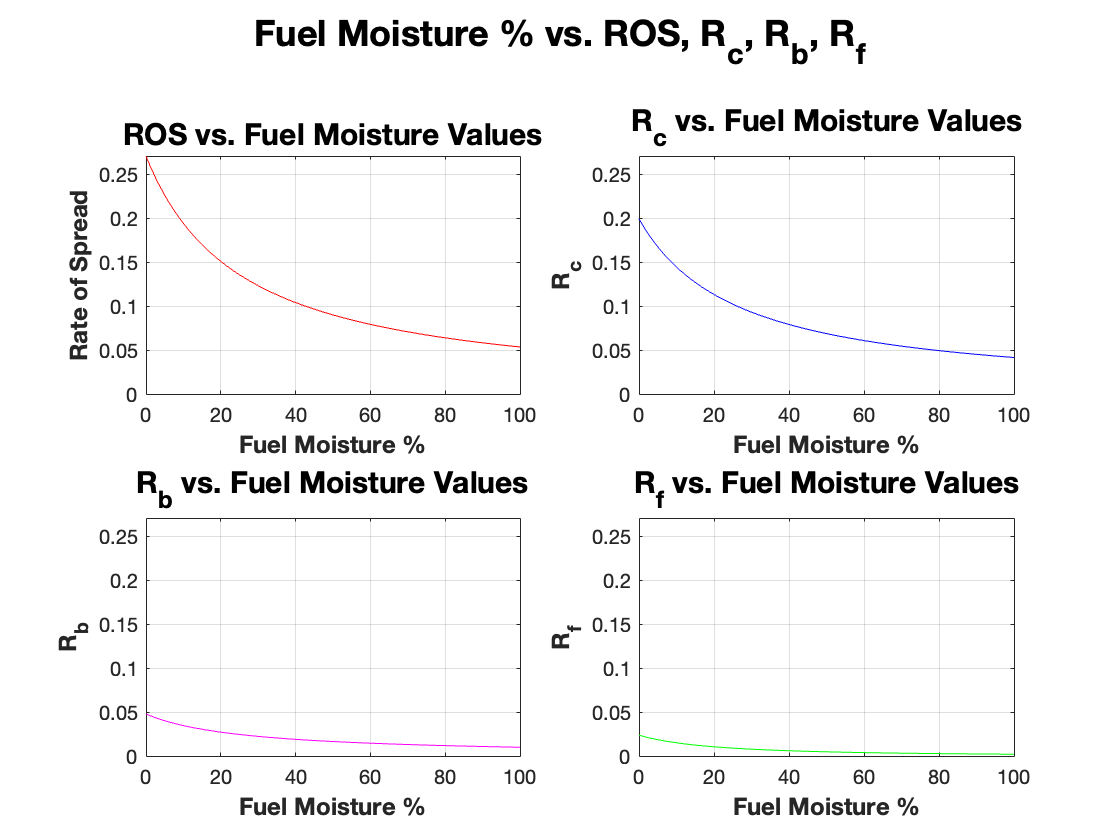
\includegraphics[scale = 0.30]{/Users/jeremybenik/Research_Files/164/Assignments/draft/Images/Balbi/FMC_with_slope.png}
  \caption{Comparison of the Balbi model and Rothermel model under varying fuel moistures}
  \label{FMC}
\end{figure}
\subsubsection*{FMC with slope and wind}
\indent In Figure \ref{FMC} there is a decrease in the ROS with an increasing fuel moisture. With more moisture in the fuel, that means more energy is required to dry out the fuel so it can burn, which slows down the rate of spread. Something to note here is that the FMC in the Rothermel model only goes to about 12$\%$. In the model there is the fuel moisture of extinction parameter and that will start causing the model to result in negative values if the fuel moisture is greater than the fuel moisture of extinction. There are many components involved in the fuel moisture calculation in the Rothermel model and their overall influence on the ROS can be seen in Figure \ref{FMC}. The moisture damping coefficient, reaction intensity, and optimum reaction velocity all decrease with an increase in the fuel moisture. The Balbi model's ROS also decreases with an increase in FMC. Since this experiment contained both wind and slope, both $R_C$ and $R_f$ contributed to the overall ROS. Unlike with the previous plots $R_b$ decreased with an increase in FMC. To further evaluate the changes from FMC, further tests were done and can be seen in Figure \ref{balbi_vs_rother_fmc_no_wind_no_slope} where the experiment occurred under no slope and no winds conditions, and Figure \ref{rothermel_neg}. \\
\subsubsection*{Fuel Moisture Without Wind and Slope}
% Fuel Moisture Without Slope
\begin{figure}
\centering
  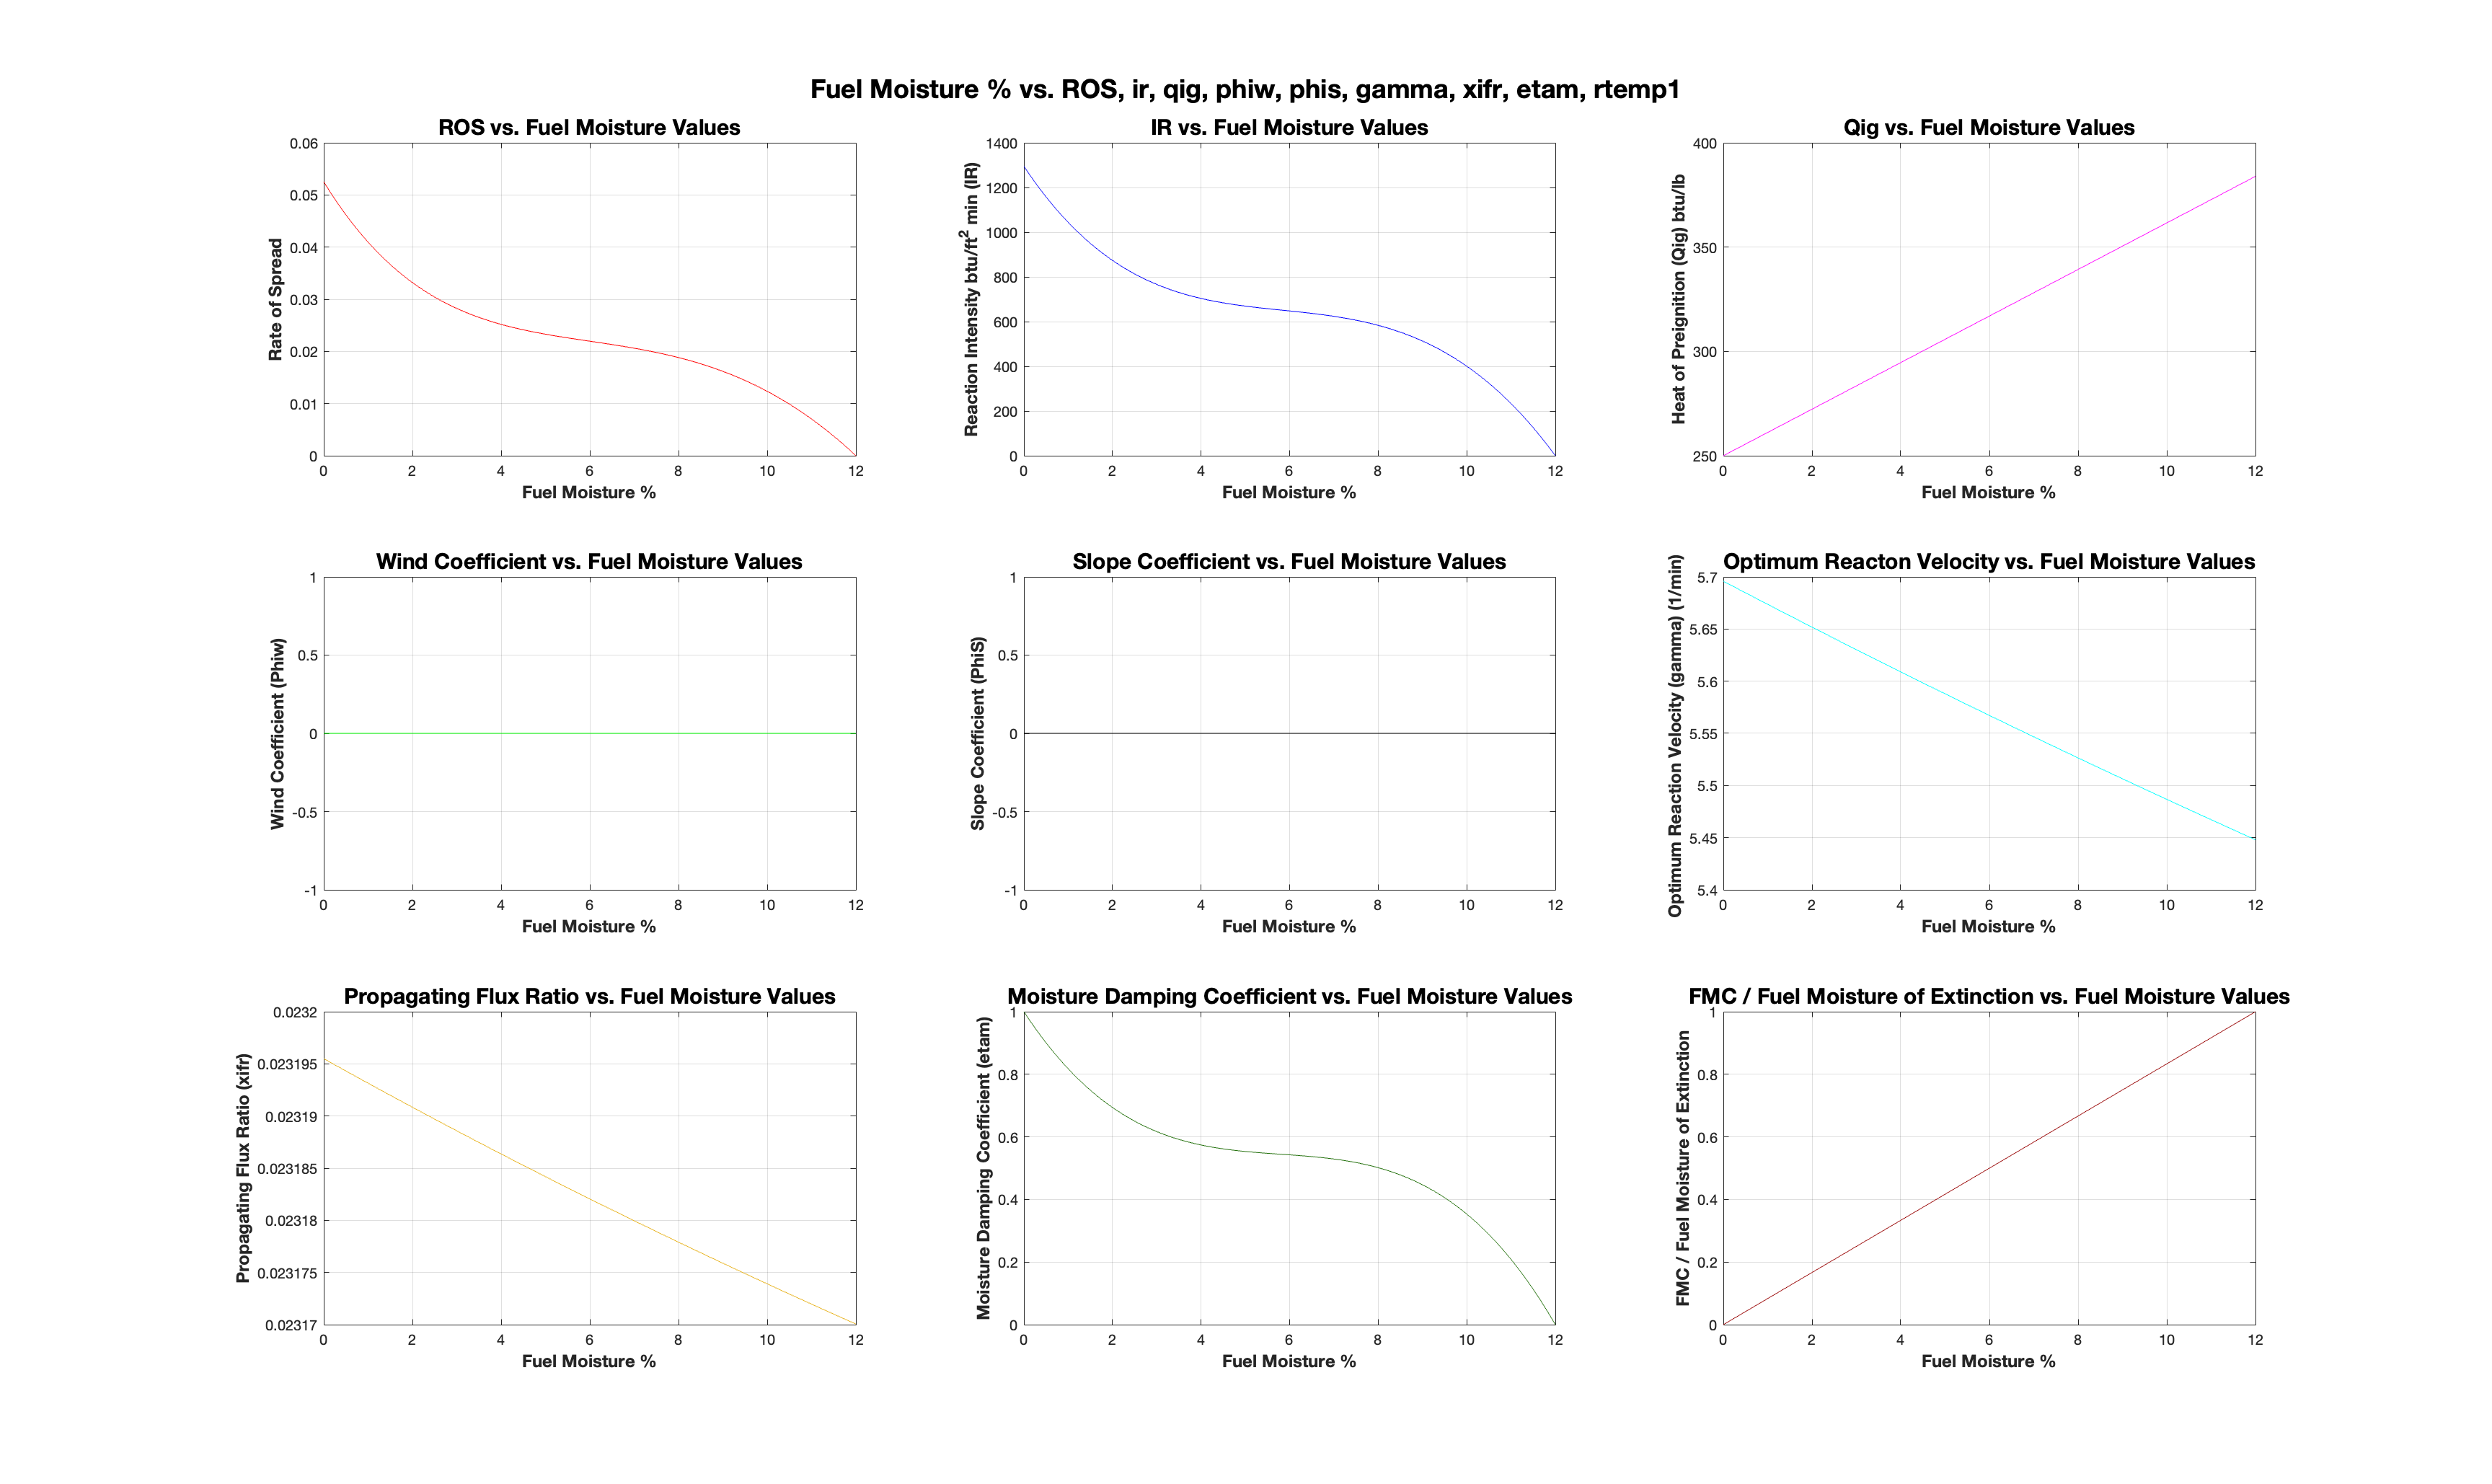
\includegraphics[scale = 0.10]{/Users/jeremybenik/Research_Files/164/Assignments/draft/Images/Rothermel/FMC_no_slope_no_wind.png}
  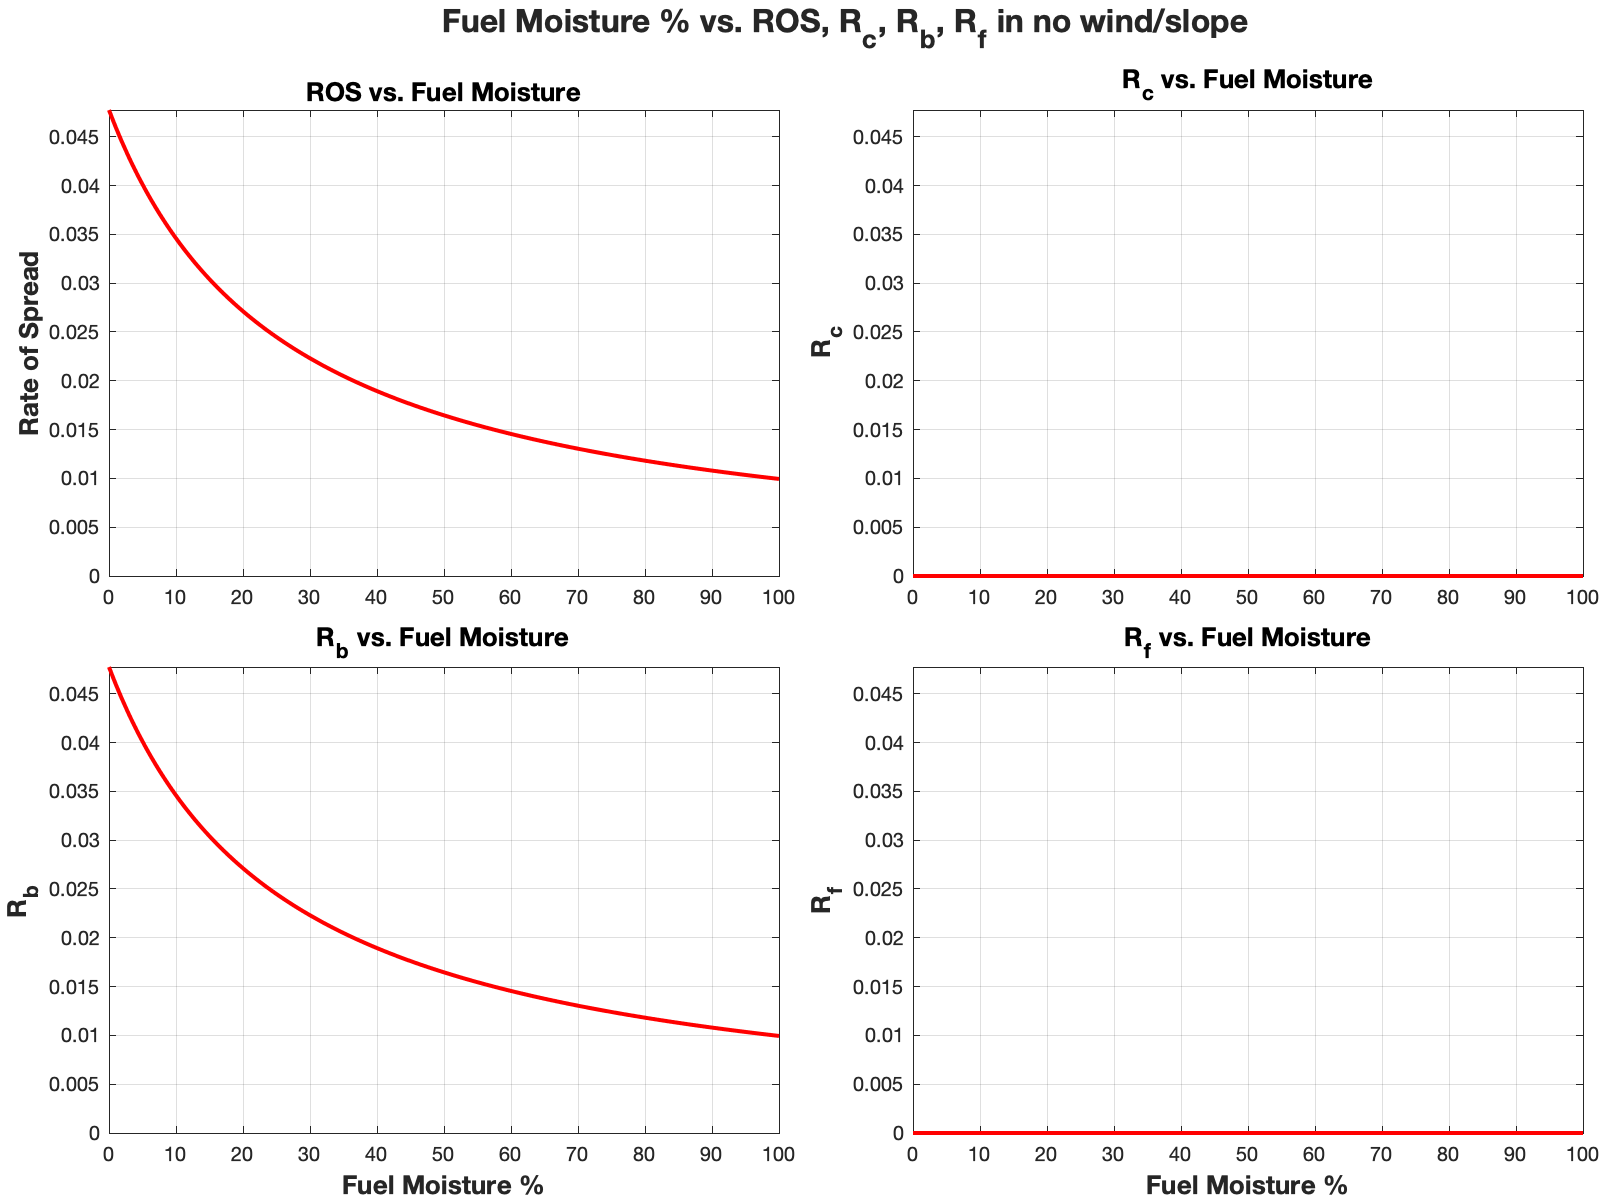
\includegraphics[scale = 0.20]{/Users/jeremybenik/Research_Files/164/Assignments/draft/Images/Balbi/FMC_without_slope_and_wind.png}
  \caption{Comparison of the Balbi model and Rothermel model under varying fuel moistures without wind or slope}
  \label{balbi_vs_rother_fmc_no_wind_no_slope}
\end{figure}

\indent Figure \ref{balbi_vs_rother_fmc_no_wind_no_slope} plots the FMC under no wind and no slope conditions to see how the ROS changes with just the FMC. Overall the ROS has decreased in both plots which is to be expected since there is no longer any preheating from convection or flame body radiation. Instead the base radiation is the only contributor to the ROS. Like in \ref{FMC}

\begin{figure}
\centering
  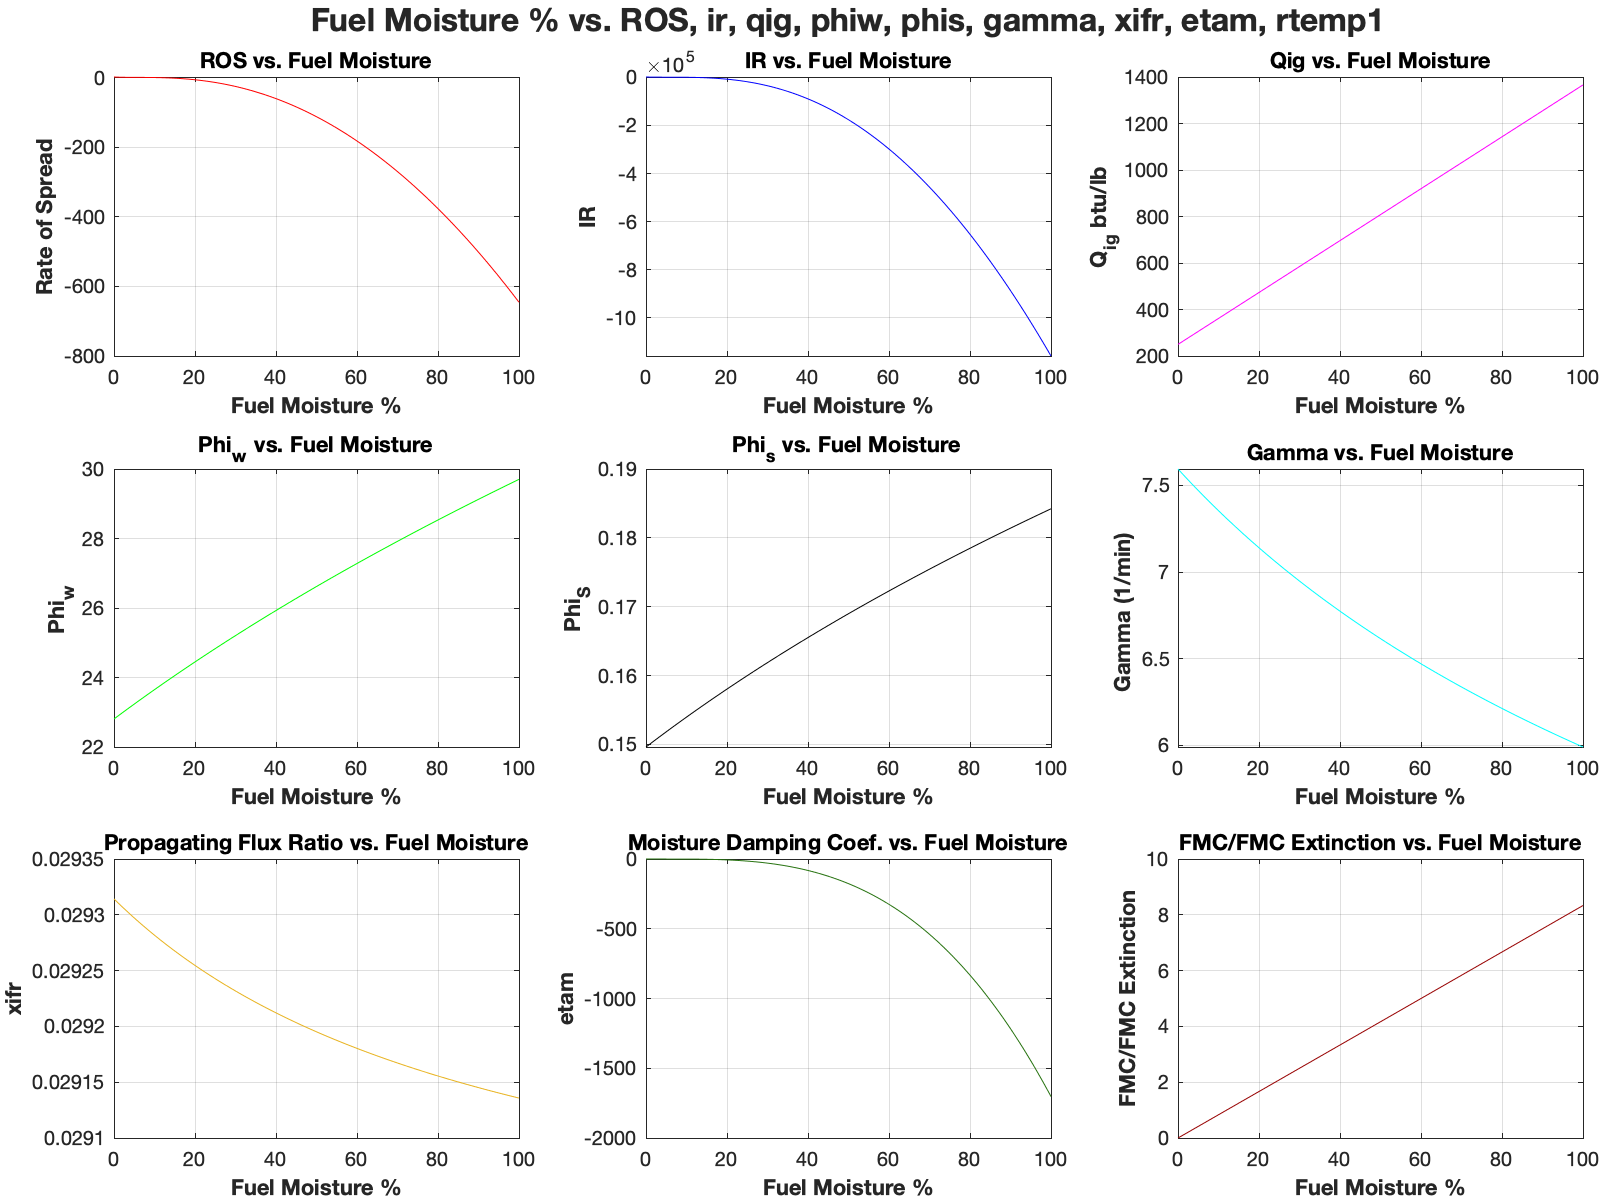
\includegraphics[scale = 0.10]{/Users/jeremybenik/Research_Files/164/Assignments/draft/Images/Rothermel/FMC_Rothermel_negative_vals.png}
  \caption{Rothermel Model FMC with fuel moisture of extinction in mind}
  \label{rothermel_neg}
\end{figure}





% Fuel Height
\subsubsection{Fuel Height}
\begin{figure}
\centering
  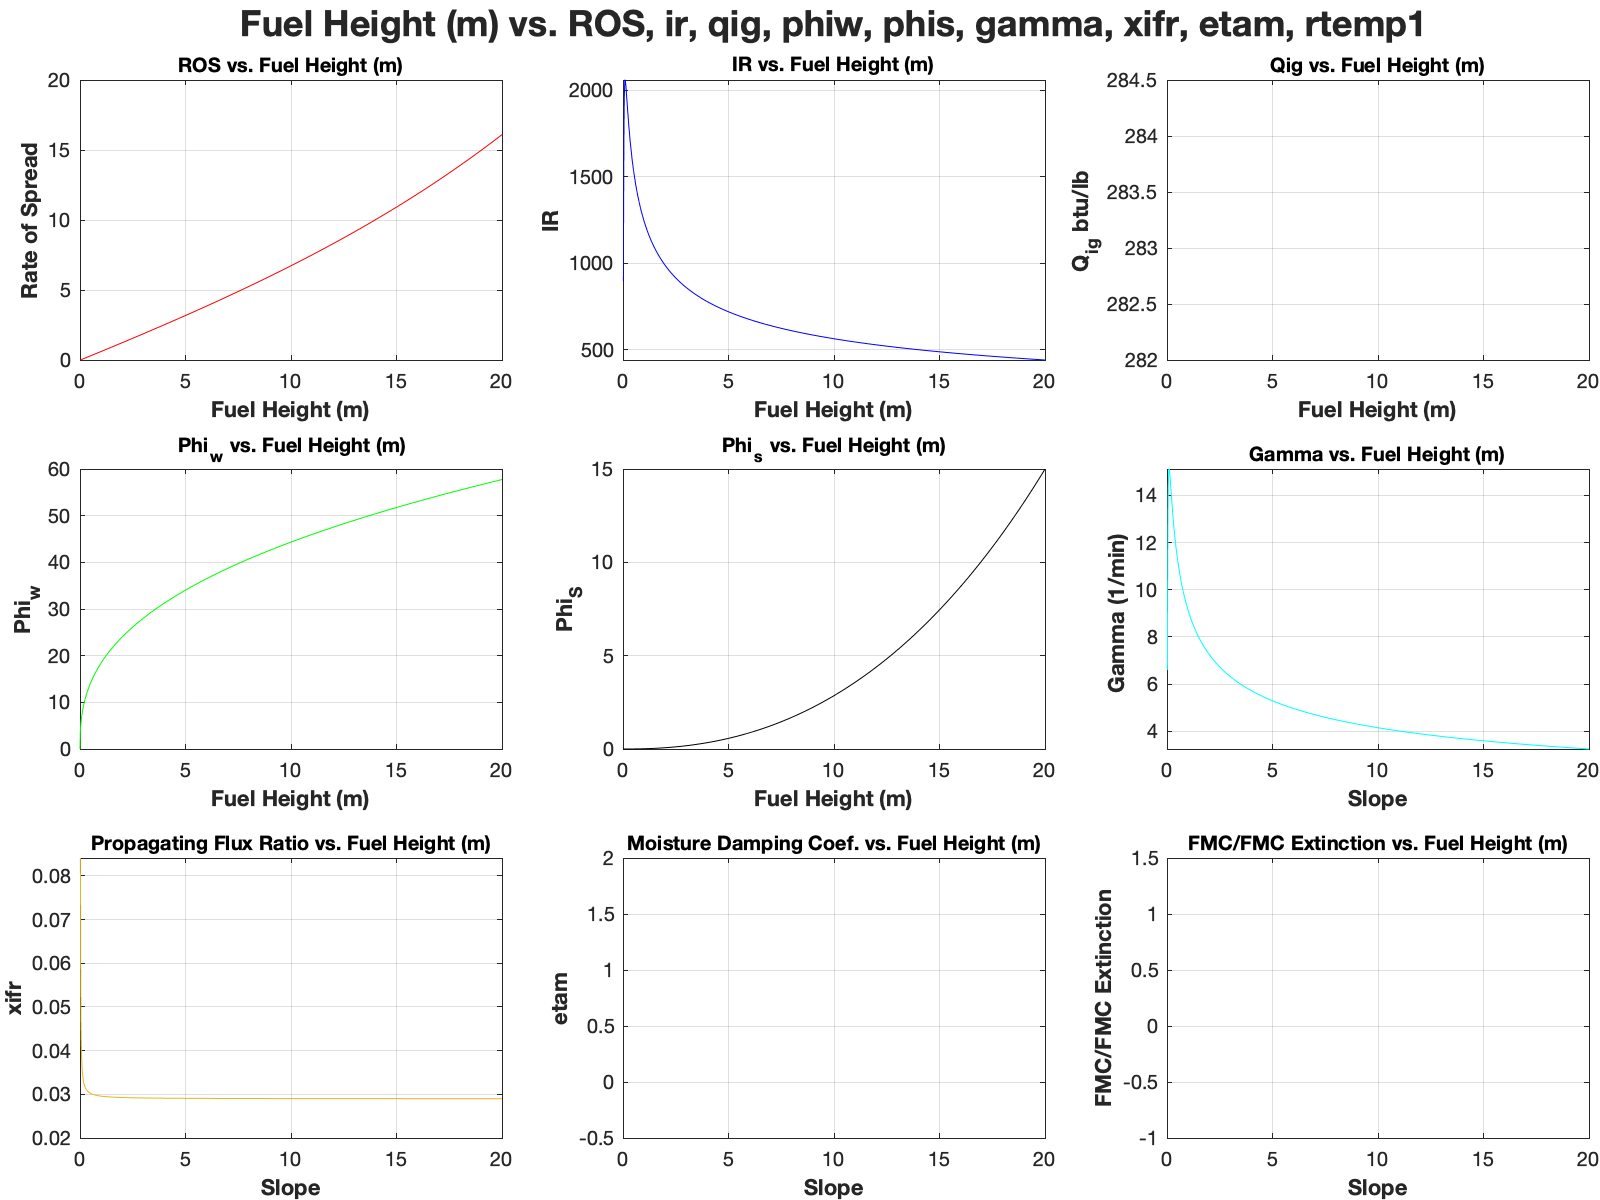
\includegraphics[scale = 0.10]{/Users/jeremybenik/Research_Files/164/Assignments/draft/Images/Rothermel/fuel_height_rothermel.png}
  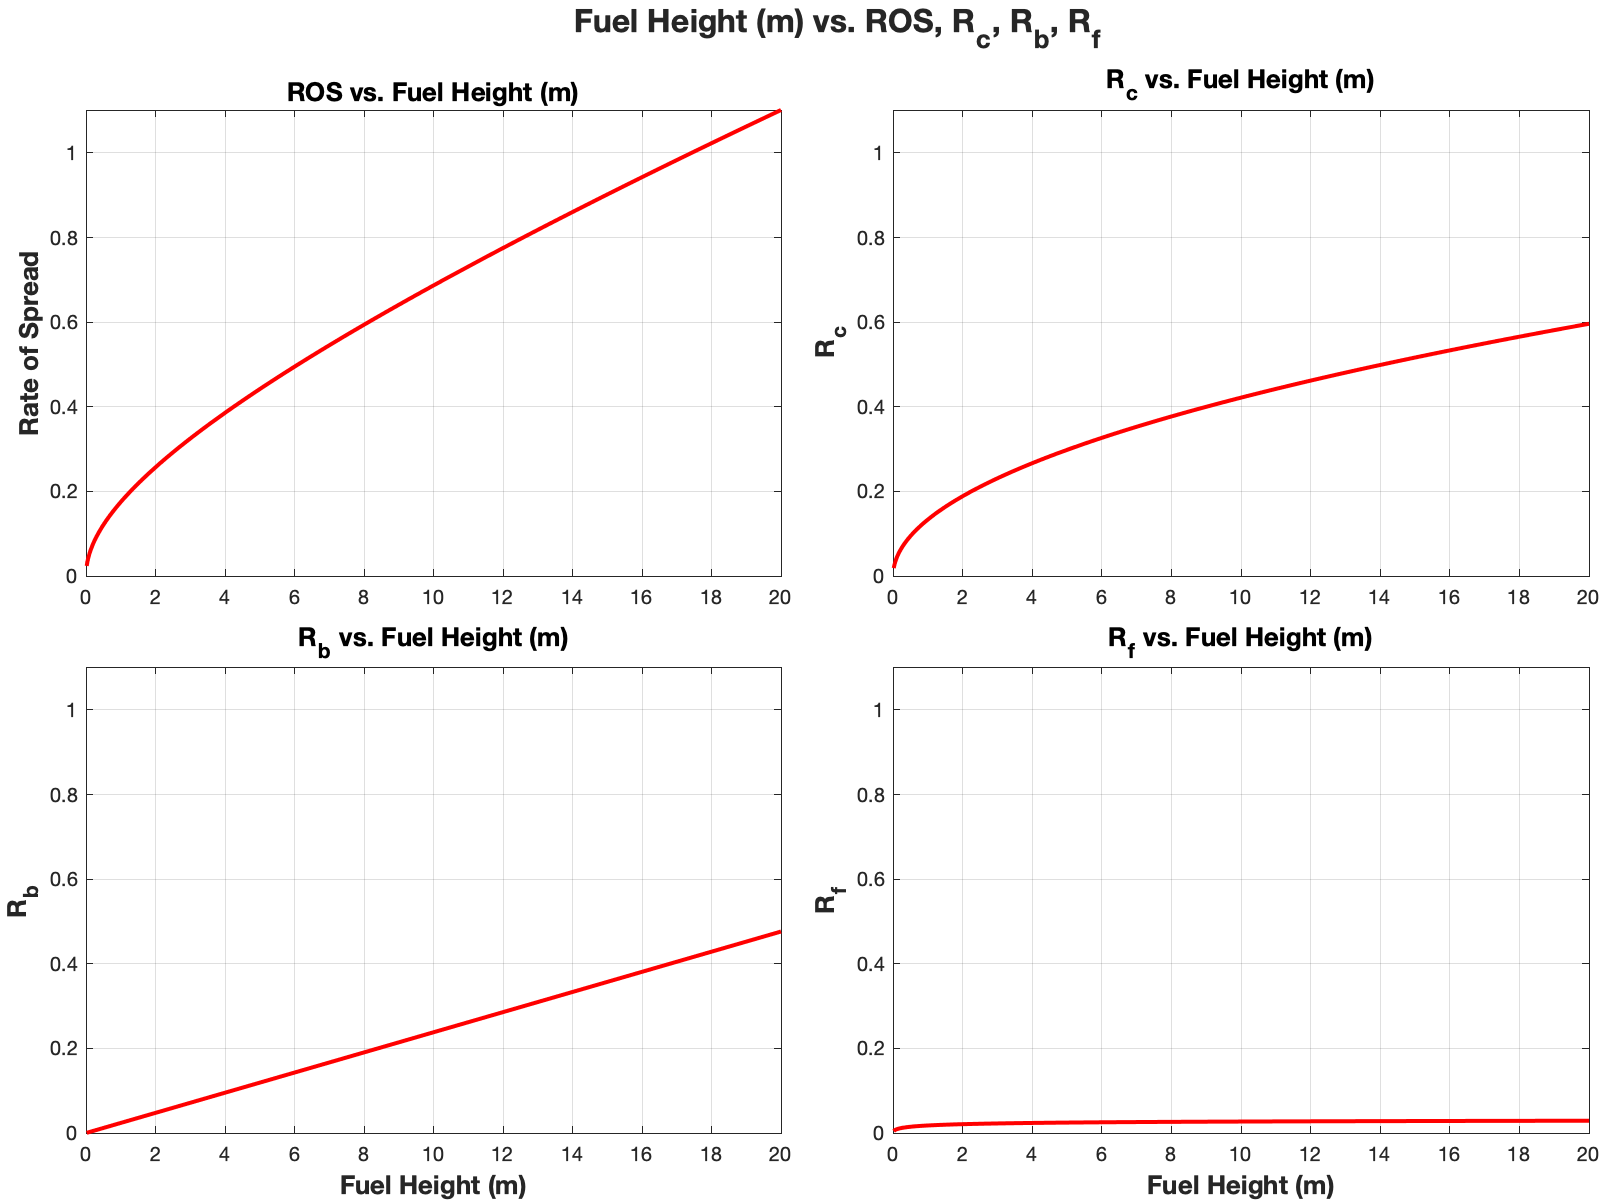
\includegraphics[scale = 0.20]{/Users/jeremybenik/Research_Files/164/Assignments/draft/Images/Balbi/fuel_depth_m.png}
  \caption{Comparison of the Balbi model and Rothermel model under varying fuel moistures without wind or slope}
  \label{balbi_vs_rother_fmc_no_wind_no_slope}
\end{figure}






















\section{Discussion}




Comparison between the semi-empirical Rothermel fire spread model and 1D physical Balbi fire spread model. This project will include the analysis of the fundamental concepts and assumptions behind these models and analysis of the results under various fuel and weather conditions.











\section{References}
\end{document}